\documentclass[12pt, titlepage]{article}

\usepackage{booktabs}

\usepackage{amsmath, mathtools}
\usepackage{amsfonts}
\usepackage{amssymb}
\usepackage{graphicx}
\usepackage{colortbl}
\usepackage{xr}
\usepackage{hyperref}
\usepackage{longtable}
\usepackage{xfrac}
\usepackage{tabularx}
\usepackage{float}
\usepackage{siunitx}
\usepackage{booktabs}
\usepackage{pdflscape}
\usepackage{afterpage}
\usepackage{float}
\usepackage{fancyvrb}
\usepackage{lscape}
\usepackage{relsize}
\usepackage{listings}
\usepackage{caption}
\usepackage{subcaption}


\usepackage[round]{natbib}
\hypersetup{
    colorlinks,
    citecolor=black,
    filecolor=black,
    linkcolor=red,
    urlcolor=blue
}
\usepackage[round]{natbib}

%% Comments

\usepackage{color}

\newif\ifcomments\commentstrue

\ifcomments
\newcommand{\authornote}[3]{\textcolor{#1}{[#3 ---#2]}}
\newcommand{\todo}[1]{\textcolor{red}{[TODO: #1]}}
\else
\newcommand{\authornote}[3]{}
\newcommand{\todo}[1]{}
\fi

\newcommand{\wss}[1]{\authornote{blue}{SS}{#1}}
\newcommand{\wpa}[1]{\authornote{magenta}{PA}{#1}}


\newcommand{\famname}{LODES} % PUT YOUR PROGRAM NAME HERE
\newcommand{\famdesc}{Library of ODE Solvers}
\newcommand{\famurl}{https://github.com/aoananp/cas741/}

\newcounter{tnum} %Test Number
\newcommand{\ttheccnum}{T\thetnum}
\newcommand{\tref}[1]{T\ref{#1}}

\usepackage{fullpage}

\begin{document}

\title{Test Report: \famdesc{} (\famname{})} 
\author{Paul Aoanan}
\date{\today}
	
\maketitle

\pagenumbering{roman}

\section{Revision History}

\begin{tabularx}{\textwidth}{p{3cm}p{2cm}X}
\toprule {\bf Date} & {\bf Version} & {\bf Notes}\\
\midrule
\today & 1.0 & Initial draft.\\
%Date 2 & 1.1 & Notes\\
\bottomrule
\end{tabularx}

~\newpage

\section{Symbols, Abbreviations and Acronyms}

\subsection{Table of Symbols}

The table that follows summarizes the symbols used in this document along with
their units.  The choice of symbols was made to be consistent with the numeral analysis
and ordinary differential equation literature and with existing documentation
for solving ordinary differential equations.  The symbols are listed in alphabetical order.

\renewcommand{\arraystretch}{1.2}
\noindent \begin{longtable*}{l l l p{8cm}} \toprule
\textbf{symbol} & \textbf{unit} & \textbf{type} & \textbf{description}\\
\midrule
$dy/dx$ & \text {-} & $\mathbb{R}$ & Rate of change of $y$ with respect to $x$\\
$\varepsilon_\text{relative}$ & - & $\mathbb{R}$ & The relative error\\
$F$ & \text{-} & $\mathbb{R}^3 \rightarrow \mathbb{R}$ & Order function applied to the Runge Kutta Method\\
$f(x, y)$ & \text{-} & $\mathbb{R}^2 \rightarrow \mathbb{R}$& Explicit form of the ODE function containing $(x,y)$\\
$f_{x}(x, y)$ & \text{-} & $\mathbb{R}^2 \rightarrow \mathbb{R}$ & Explicit form of the derivative of $f(x, y)$ with respect to x\\
$f_{y}(x, y)$ & \text{-} & $\mathbb{R}^2 \rightarrow \mathbb{R}$ & Explicit form of the derivative of $f(x, y)$ with respect to y\\
$h$ & \text{-} & $\mathbb{R}$ . $h > 0$ & Step-size from $x_\text{(0)}$ to the next point $x_\text{(1)}$, where $x_\text{(1)} = x_\text{(0)} + h$\\
$K_1, K_2, K_3, K_4$ & $\mathbb{R}$ & \text{-} & Intermediary variables used in the Runge-Kutta method\\
$n$ & \text{-} & $\mathbb{R}$ & Reference recursion step\\
$o$ & \text{-} & $\mathbb{R}$  & Solution variable\\
T & - & - & Test\\
$x_\text{0}$ & \text{-} & $\mathbb{R}$  & Initial value $x$\\
$x_\text{k}$ & \text{-} & $\mathbb{R}$  & Final value $x$\\
$x_\text{n}$ & \text{-} & $\mathbb{R}$ & Intermediate $n^\text{th}$ value $x$\\
$y_\text{0}$ & \text{-} & $\mathbb{R}$ & Initial value $y$\\ 
$y_\text{k}$ & \text{-} & $\mathbb{R}$  & Final value $y$\\
$y_\text{n}$ & \text{-} &$\mathbb{R}$ & Intermediate $n^\text{th}$ value $y$\\ 
$y'$ & \text{-} &$\mathbb{R} \rightarrow \mathbb{R}$& Implicit form of the first order ODE = $f(x, y)$\\
$y^\text{(n)}$ & \text{-} &$\mathbb{R} \rightarrow \mathbb{R}$& Implicit form of the ODE to the $n^\text{th}$ order\\
$y$ & \text{-} & $1$ x $\mathbb{R}^k$ & The array containing all intermediate $y_\text{n}$ values\\
\bottomrule
\end{longtable*}

%\wss{symbols, abbreviations or acronyms -- you can reference the SRS tables if needed}

\newpage

\tableofcontents

\listoftables %if appropriate

\listoffigures %if appropriate

\newpage

\pagenumbering{arabic}

\section{Introduction}

This document serves as the Test Report for the \famdesc{} (\famname{}) which 
lays out in detail the results of the execution of the \famname{} Test Plan.
The requirements for the software are described in the \famname{} Software
Requirements Specification. The aim of the Test Report is to document and show that
\famname{} produces accurate and valid (in the scope of detailed in the SRS and Test Plan) results.\\

The Overview (Section \ref{sec_overview}) discusses how testing
slightly deviates from the Test Plan in its execution.

The following sections describe the evaluation of the software against the
Functional Requirements (Section \ref{sec_fr}), Non-Functional Requirements
(Section \ref{sec_nfr}). It will also compare \famname{}
to existing software in Comparison to Existing Implementation (Section \ref{sec_comp_exist_imp}).\\

In the sections after, Unit Testing (Section \ref{sec_ut}),
Changes Due to Testing (Section \ref{sec_changes}), Automated Testing (Section \ref{sec_at}),
Trace to Requirements (Section \ref{sec_trace_req}), Trace to Modules (Section \ref{sec_trace_modules},
and Code Coverage Metrics (Section \ref{sec_ccm}) are discussed.\\

\section{Overview} \label{sec_overview}
The Test Report documents the results of the tests
carried out to verify the behaviour of the
\famname{} software. The Test Plan suggests that it should carry out testing such that
that the test report shall describe and analyze the numerical differences of the hand-executed
solution to the numerical analysis methods versus the solutions obtained from \famname{}.
This Test Report carries out the tests, with the same intent of verification, and instead of
only comparing against the hand-executed solution, it compares the results with
the MATLAB generated solutions as well.

\newpage

\section{Functional Requirements Evaluation} \label{sec_fr}
\subsection{Calculation Tests}
\subsubsection{Simple Cases: T-1, T-5, T-9, T-13}
Input: $f(x,y) = y, h = 2,x_0 = 0,y_0 = 1,x_k = 2$\\

\textbf{Test Plan Test Case: T-1}\\
Expected output: The value of $y_k = 3$. This test passes.\\
\begin{figure}[H]
 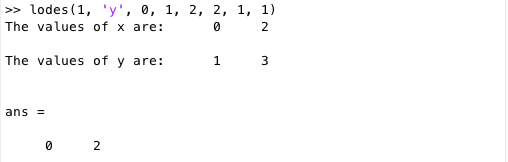
\includegraphics[width=\linewidth]{images/T1}
  \caption{T-1 result.}
  \label{fig:T1}
\end{figure}

\textbf{Test Plan Test Case: T-5}\\
Expected output: The value of $y_k = 5$. This test passes.\\
\begin{figure}[H]
 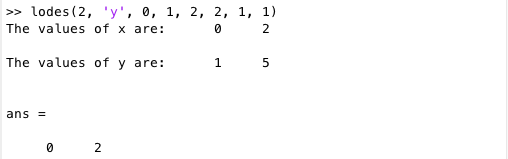
\includegraphics[width=\linewidth]{images/T5}
  \caption{T-5 result.}
  \label{fig:T5}
\end{figure}

\textbf{Test Plan Test Case: T-9}\\
Expected output: The value of $y_k = 5$. This test passes.\\
\begin{figure}[H]
 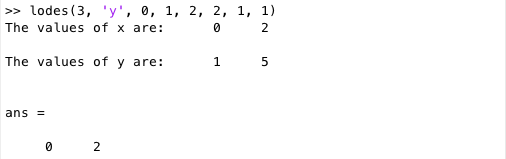
\includegraphics[width=\linewidth]{images/T9}
  \caption{T-9 result.}
  \label{fig:T9}
\end{figure}

\textbf{Test Plan Test Case: T-13}\\
Expected output: The value of $y_k = 7$. This test passes.\\
\begin{figure}[H]
 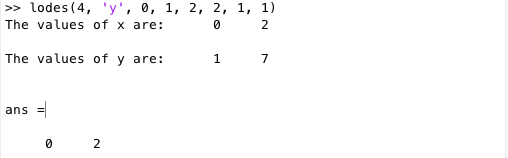
\includegraphics[width=\linewidth]{images/T13}
  \caption{T-13 result.}
  \label{fig:T13}
\end{figure}

\subsubsection{Simple-Iterative Cases: T-2, T-6, T-10, T-14}
Input: $f(x,y) = y, h = 0.5, x_0 = 0,y_0 = 1,x_k = 2$\\

\textbf{Test Plan Test Case: T-2}\\
Expected output: The value of $y_k = 5.0625$. This test passes.\\
\begin{figure}[H]
 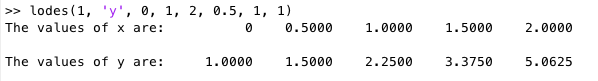
\includegraphics[width=\linewidth]{images/T2}
  \caption{T-2 result.}
  \label{fig:T2}
\end{figure}

\textbf{Test Plan Test Case: T-6}\\
Expected output: The value of $y_k = 6.9729$. This test passes.\\
\begin{figure}[H]
 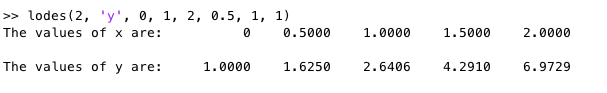
\includegraphics[width=\linewidth]{images/T6}
  \caption{T-6 result.}
  \label{fig:T6}
\end{figure}

\textbf{Test Plan Test Case: T-10}\\
Expected output: The value of $y_k = 6.9729$. This test passes.\\
\begin{figure}[H]
 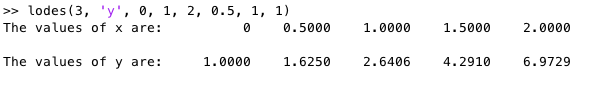
\includegraphics[width=\linewidth]{images/T10}
  \caption{T-10 result.}
  \label{fig:T10}
\end{figure}

\textbf{Test Plan Test Case: T-14}\\
Expected output: The value of $y_k = 7.38340$. This test passes.\\
\begin{figure}[H]
 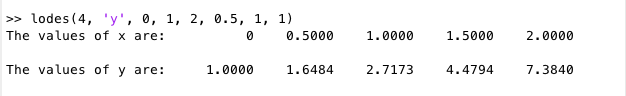
\includegraphics[width=\linewidth]{images/T14}
  \caption{T-14 result.}
  \label{fig:T14}
\end{figure}

\subsubsection{Linear Trigonometric Cases: T-3, T-7, T-11, T-15}
Input: $f(x,y) = y, h = 5, x_0 = 0,y_0 = 1,x_k = 5$\\

\textbf{Test Plan Test Case: T-3}\\
Expected output: The value of $y_k = -4$. This test passes.\\
\begin{figure}[H]
 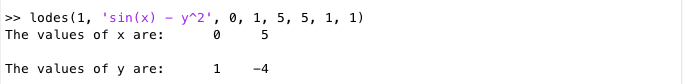
\includegraphics[width=\linewidth]{images/T3}
  \caption{T-3 result.}
  \label{fig:T3}
\end{figure}

\textbf{Test Plan Test Case: T-7}\\
Expected output: The value of $y_k = -43.8973$. This test passes.\\
\begin{figure}[H]
 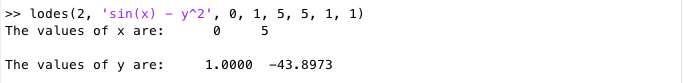
\includegraphics[width=\linewidth]{images/T7}
  \caption{T-7 result.}
  \label{fig:T7}
\end{figure}

\textbf{Test Plan Test Case: T-11}\\
Expected output: The value of $y_k = -43.8973$. This test passes.\\
\begin{figure}[H]
 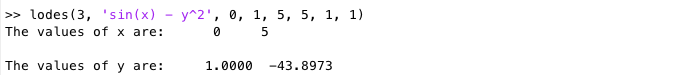
\includegraphics[width=\linewidth]{images/T11}
  \caption{T-11 result.}
  \label{fig:T11}
\end{figure}

\textbf{Test Plan Test Case: T-15}\\
Expected output: The value of $y_k = -1702.8$. This test passes.\\
\begin{figure}[H]
 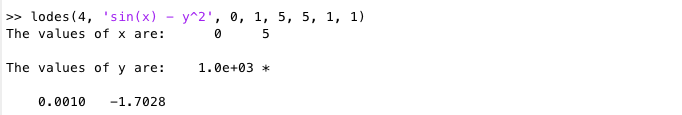
\includegraphics[width=\linewidth]{images/T15}
  \caption{T-15 result.}
  \label{fig:T15}
\end{figure}

\subsubsection{Linear Trigonometric Iterative Cases: T-4, T-8, T-12, T-16}
Input: $f(x,y) = sin(x) - y^2, h = 1, x_0 = 0,y_0 = 1,x_k = 5$\\

\textbf{Test Plan Test Case: T-4}\\
Expected output: The value of $y_k = -0.6695$. This test passes.\\
\begin{figure}[H]
 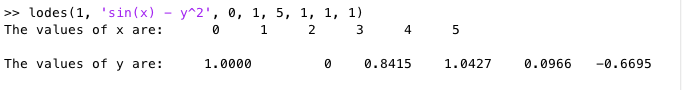
\includegraphics[width=\linewidth]{images/T4}
  \caption{T-4 result.}
  \label{fig:T4}
\end{figure}

\textbf{Test Plan Test Case: T-8}\\
Expected output: The value of $y_k = -1.1012$. This test passes.\\
\begin{figure}[H]
 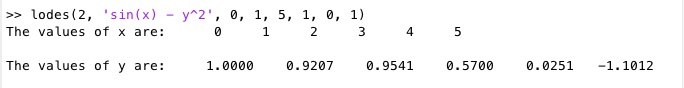
\includegraphics[width=\linewidth]{images/T8}
  \caption{T-8 result.}
  \label{fig:T}
\end{figure}

\textbf{Test Plan Test Case: T-12}\\
Expected output: The value of $y_k = -1.1012$. This test passes.\\
\begin{figure}[H]
 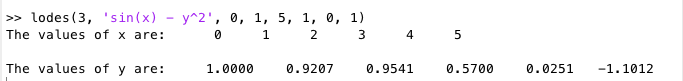
\includegraphics[width=\linewidth]{images/T12}
  \caption{T-12 result.}
  \label{fig:T12}
\end{figure}

\textbf{Test Plan Test Case: T-16}\\
Expected output: The value of $y_k = -1.0284$. This test passes.\\
\begin{figure}[H]
 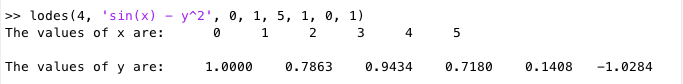
\includegraphics[width=\linewidth]{images/T16}
  \caption{T-16 result.}
  \label{fig:T16}
\end{figure}

\section{Nonfunctional Requirements Evaluation} \label{sec_nfr}
\subsection{Speed Test Plan Test Case: T-17}
Input: $f(x,y) = sin(x) - y^2, h = 1e-3, x_0 = 0,y_0 = 1,x_k = 5$\\

\textbf{Test Plan Test Case: T-17}\\
Expected output: The execution time difference of \famname{} is not greater than 4 times that of MATLAB.
This test fails as the execution time of \famname{} is 2,000 times greater than MATLAB's.\\
\begin{figure}[H]
 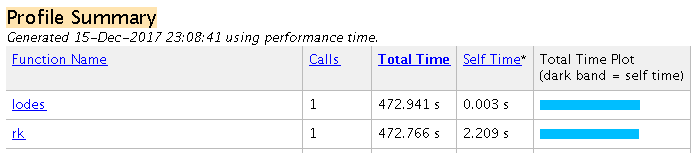
\includegraphics[width=\linewidth]{images/T17a}
  \caption{T-17 \famname{} rk() result.}
  \label{fig:T17a}
\end{figure}
\begin{figure}[H]
 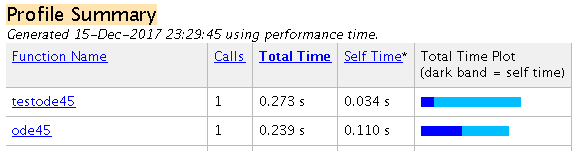
\includegraphics[width=\linewidth]{images/T17b}
  \caption{T-17 MATLAB ode45() result.}
  \label{fig:T17b}
\end{figure}

	
\section{Comparison to Existing Implementation}	 \label{sec_comp_exist_imp}

This section compares the calculation of \famname{} to MATLAB's ode45() function.\\

\textbf{Test Plan Test Case: T-18}\\
The following input parameters were tested (as above):
\begin{itemize}
\item Test 1 (\ref{sec_t1}): $f(x,y) = y, h = 2,x_0 = 0,y_0 = 1,x_k = 2$
\item Test 2 (\ref{sec_t2}): $f(x,y) = y, h = 0.5,x_0 = 0,y_0 = 1,x_k = 2$
\item Test 3 (\ref{sec_t3}): $f(x,y) = sin(x) - y^2, h = 5,x_0 = 0,y_0 = 1,x_k = 5$
\item Test 4 (\ref{sec_t4}): $f(x,y) = sin(x) - y^2, h = 1,x_0 = 0,y_0 = 1,x_k = 5$
\end{itemize}

This phase of testing is automated and the results are shown in Section \ref{app_a}.
The following equation was implemented to compare the results labeled as \textbf{norm}:
$$\epsilon_{\text{relative}} = \text{norm} = \frac{\|\text{Result}_\text{MATLAB} - \text{Result}_\text{\famname{}}\|} {\| \text{Result}
_\text{MATLAB} \|} $$

Output/Result: The $\epsilon_{\text{relative}}$ vs. $h$ plots.
The intermediate $y$ values (Result) are compared according to the following formula of the relative error norm percentage -
$$\epsilon_{\text{relative}} =100 * \frac{\text{Result}_\text{MATLAB} - \text{Result}_\text{\famname{}}} {\text{Result}
_\text{MATLAB}} $$

\subsection{Test 1: $f(x,y) = y, h = 2,x_0 = 0,y_0 = 1,x_k = 2$} \label{sec_t1}
\begin{figure}[H]
\centering
\begin{subfigure}{.55\textwidth}
  \centering
  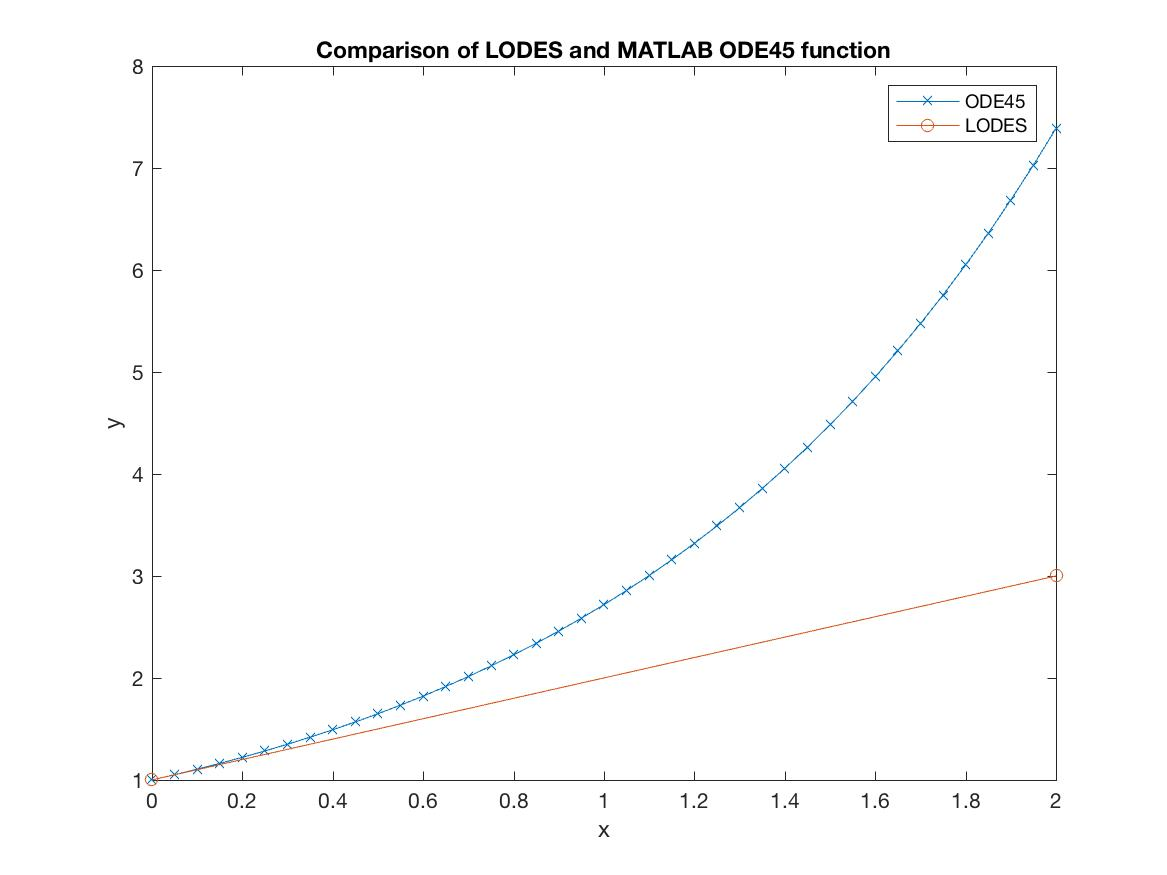
\includegraphics[width=\linewidth]{images/Test1/1LODESvsMATLABPlot.jpg}
  \caption{Euler vs. ODE45}
  \label{fig:euler1a}
\end{subfigure}%
\begin{subfigure}{.55\textwidth}
  \centering
  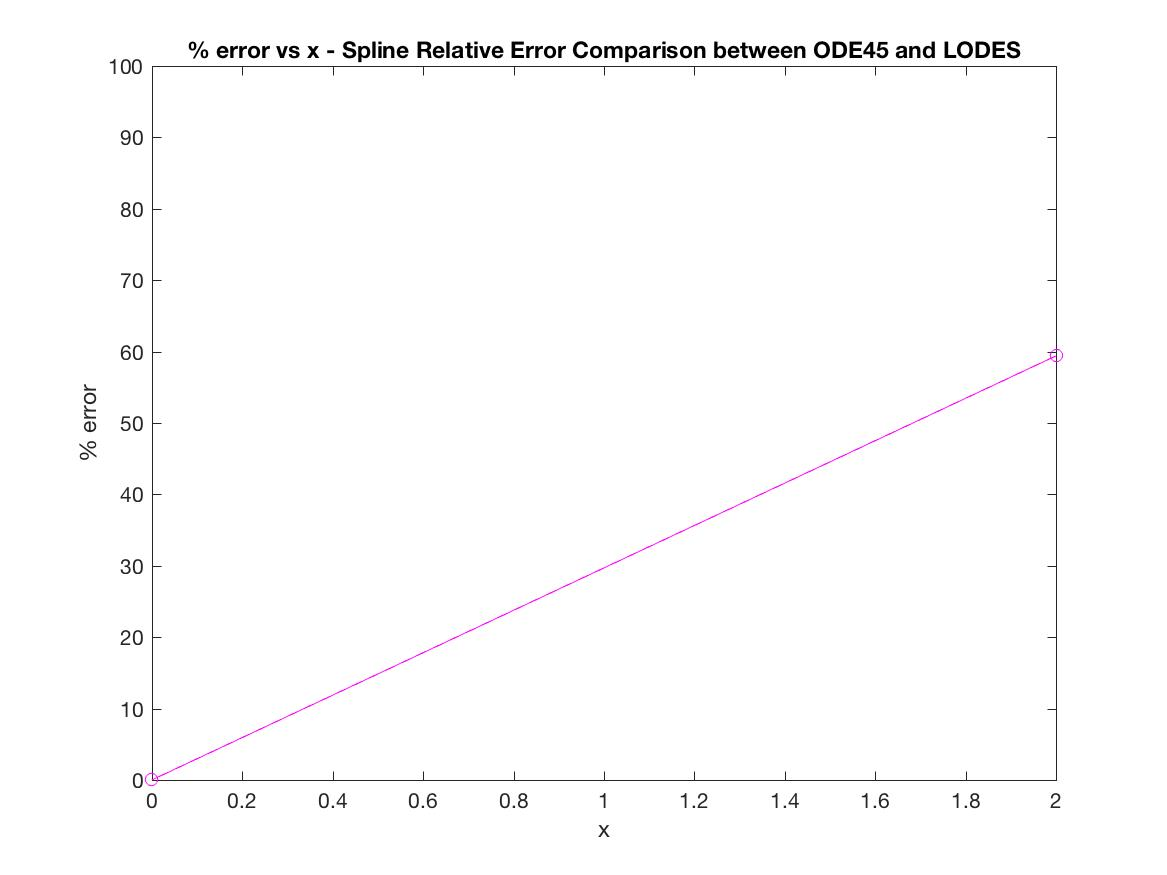
\includegraphics[width=\linewidth]{images/Test1/1RelativeErrorPlot.jpg}
  \caption{Relative Error Norm - Euler}
  \label{fig:euler1b}
\end{subfigure}
\caption{Euler's Method Analysis Graphs}
\label{fig:euler1}
\end{figure}

\begin{figure}[H]
\centering
\begin{subfigure}{.55\textwidth}
  \centering
  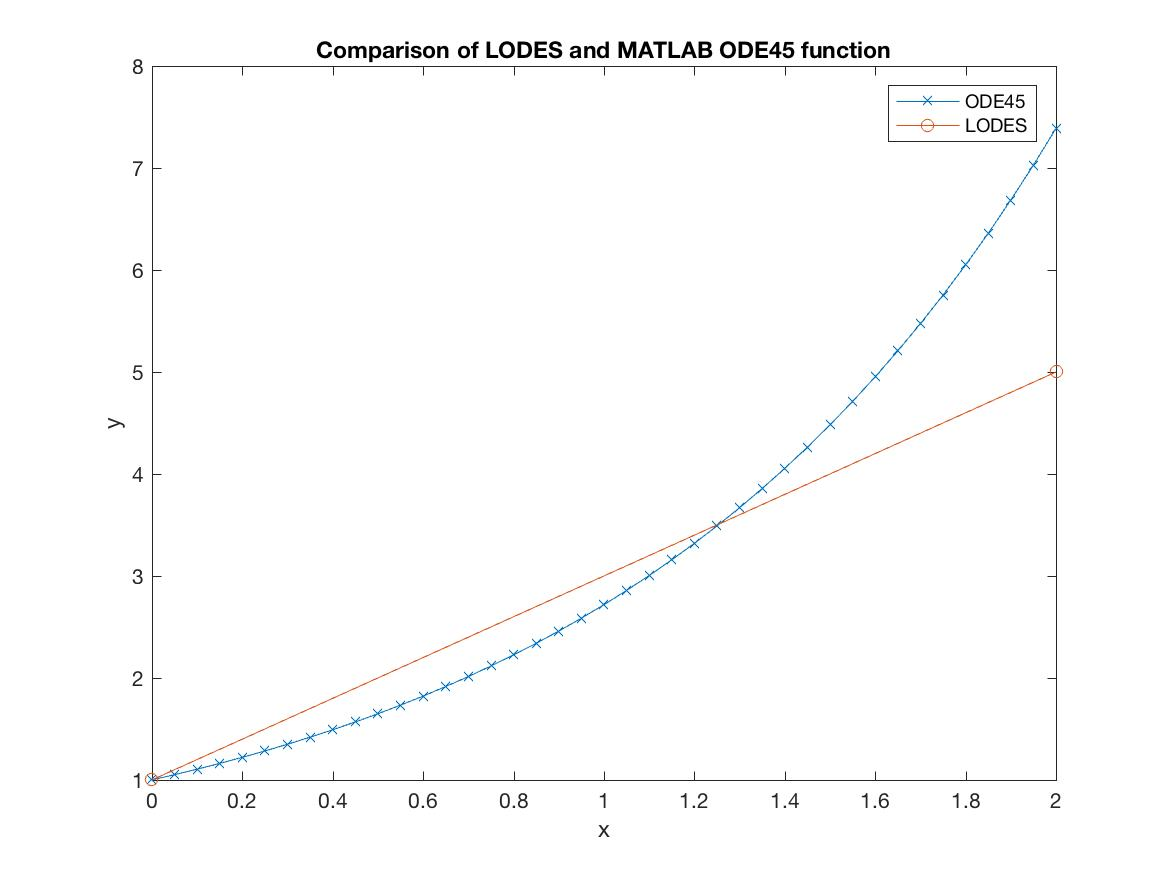
\includegraphics[width=\linewidth]{images/Test1/2LODESvsMATLABPlot.jpg}
  \caption{Trapezoid vs. ODE45}
  \label{fig:trap1a}
\end{subfigure}%
\begin{subfigure}{.55\textwidth}
  \centering
  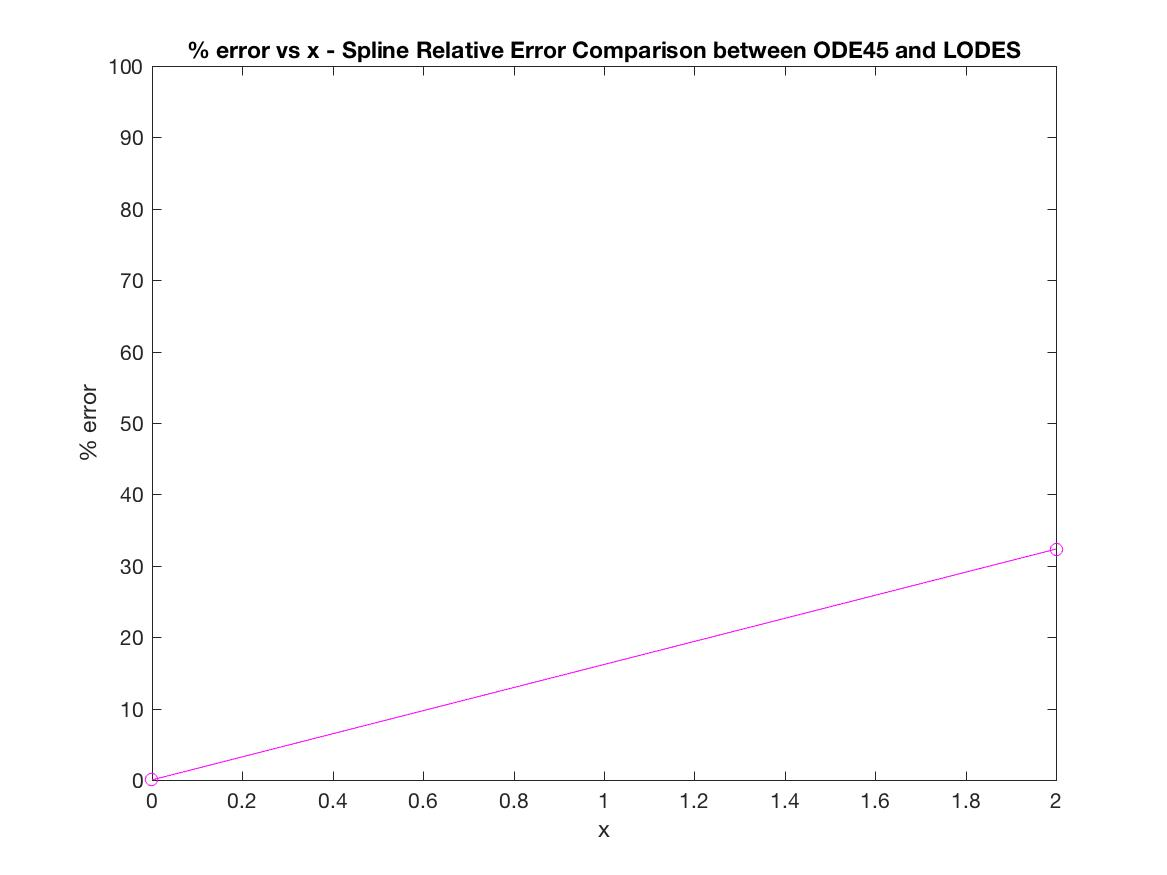
\includegraphics[width=\linewidth]{images/Test1/2RelativeErrorPlot.jpg}
  \caption{Relative Error Norm - Trapezoid}
  \label{fig:trap1b}
\end{subfigure}
\caption{Trapezoidal Method Analysis Graphs}
\label{fig:trap1}
\end{figure}

\begin{figure}[H]
\centering
\begin{subfigure}{.55\textwidth}
  \centering
  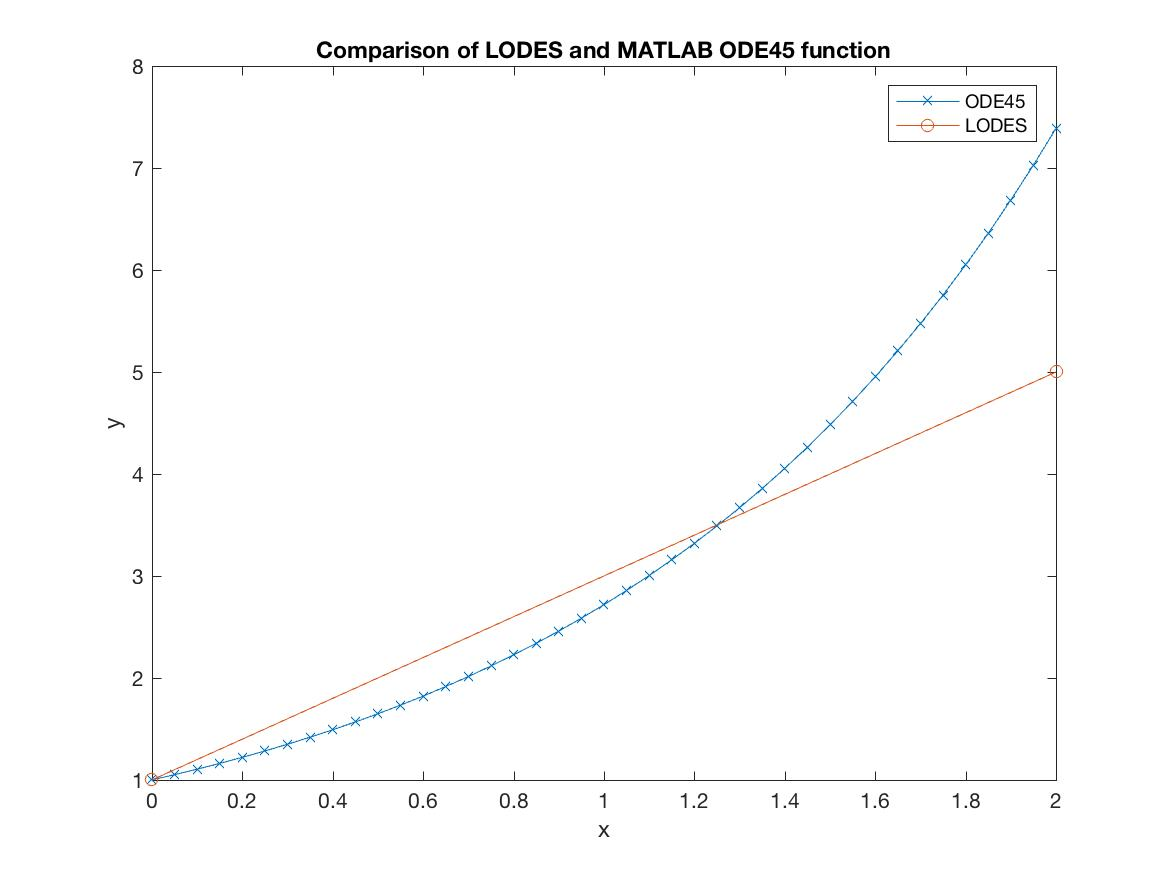
\includegraphics[width=\linewidth]{images/Test1/3LODESvsMATLABPlot.jpg}
  \caption{Heun vs. ODE45}
  \label{fig:heun1a}
\end{subfigure}%
\begin{subfigure}{.55\textwidth}
  \centering
  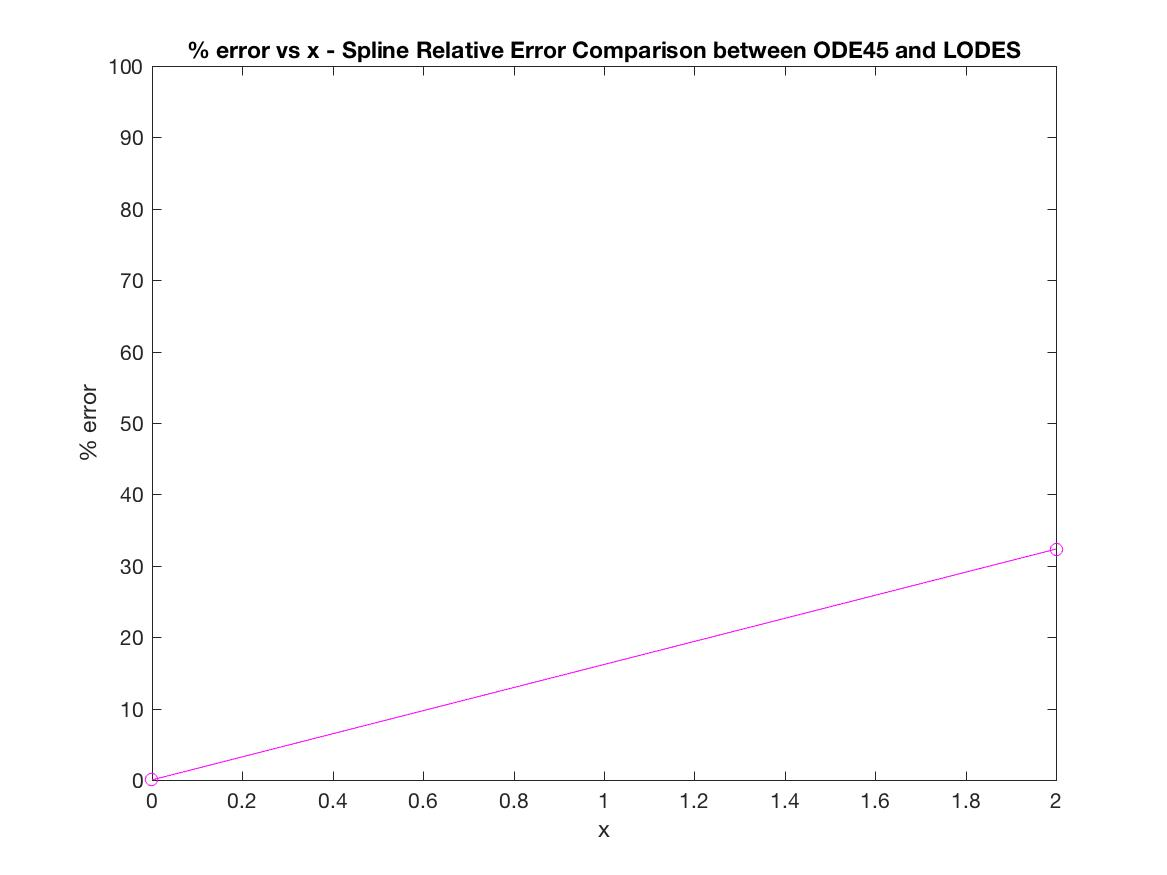
\includegraphics[width=\linewidth]{images/Test1/3RelativeErrorPlot.jpg}
  \caption{Relative Error Norm - Heun}
  \label{fig:heun1b}
\end{subfigure}
\caption{Heun's Method Analysis Graphs}
\label{fig:heun1}
\end{figure}

\begin{figure}[H]
\centering
\begin{subfigure}{.55\textwidth}
  \centering
  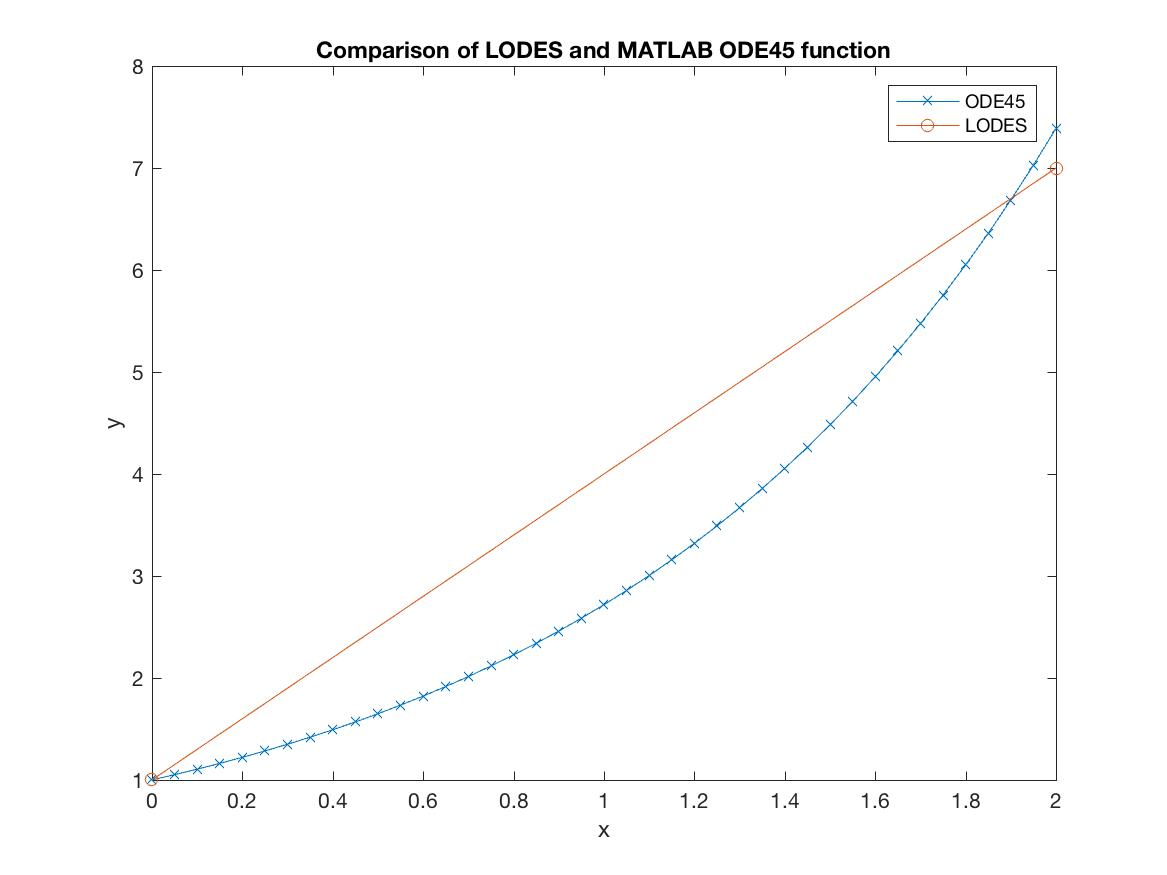
\includegraphics[width=\linewidth]{images/Test1/4LODESvsMATLABPlot.jpg}
  \caption{Runge-Kutta 4 vs. ODE45}
  \label{fig:rk1a}
\end{subfigure}%
\begin{subfigure}{.55\textwidth}
  \centering
  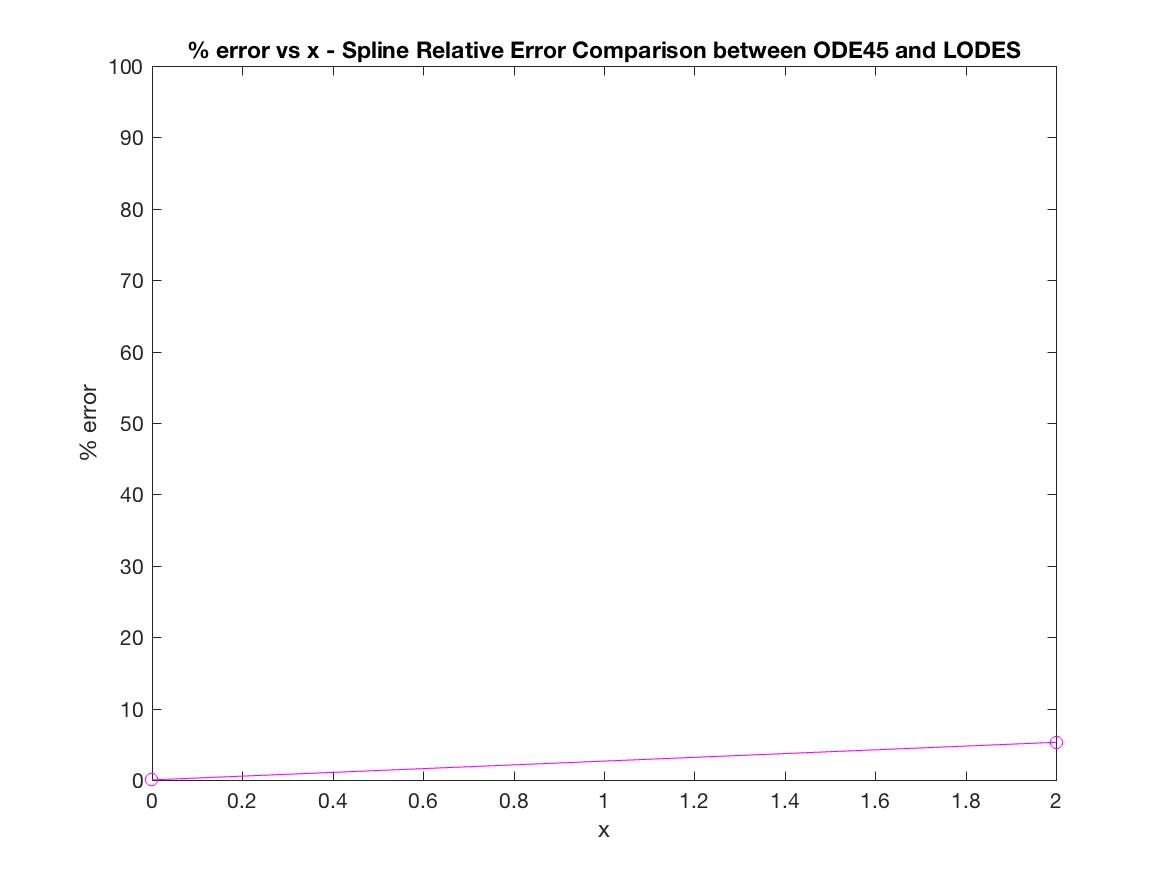
\includegraphics[width=\linewidth]{images/Test1/4RelativeErrorPlot.jpg}
  \caption{Relative Error Norm - Runge-Kutta 4}
  \label{fig:rk1b}
\end{subfigure}
\caption{Runge-Kutta 4 Method Analysis Graphs}
\label{fig:rk1}
\end{figure}



\subsection{Test 2: $f(x,y) = y, h = 0.5,x_0 = 0,y_0 = 1,x_k = 2$} \label{sec_t2}
\begin{figure}[H]
\centering
\begin{subfigure}{.55\textwidth}
  \centering
  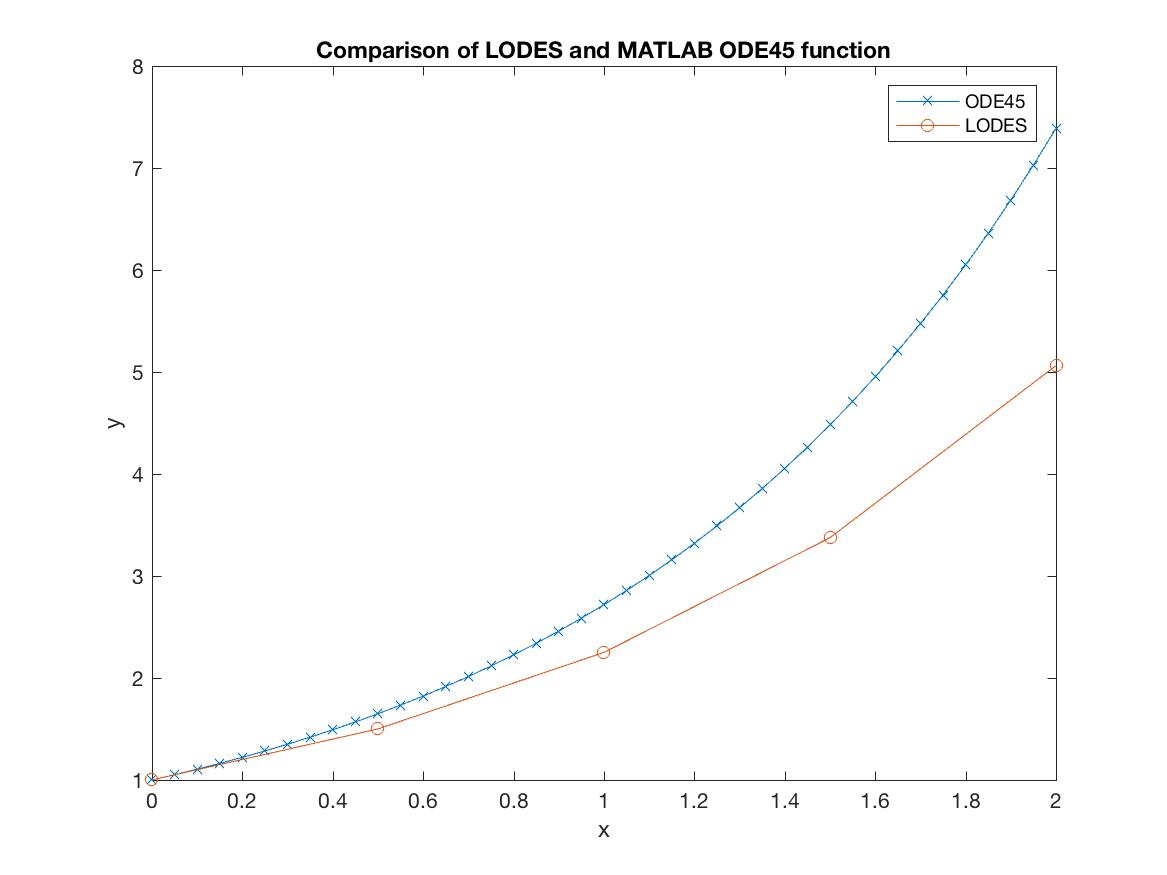
\includegraphics[width=\linewidth]{images/Test2/1LODESvsMATLABPlot.jpg}
  \caption{Euler vs. ODE45}
  \label{fig:euler2a}
\end{subfigure}%
\begin{subfigure}{.55\textwidth}
  \centering
  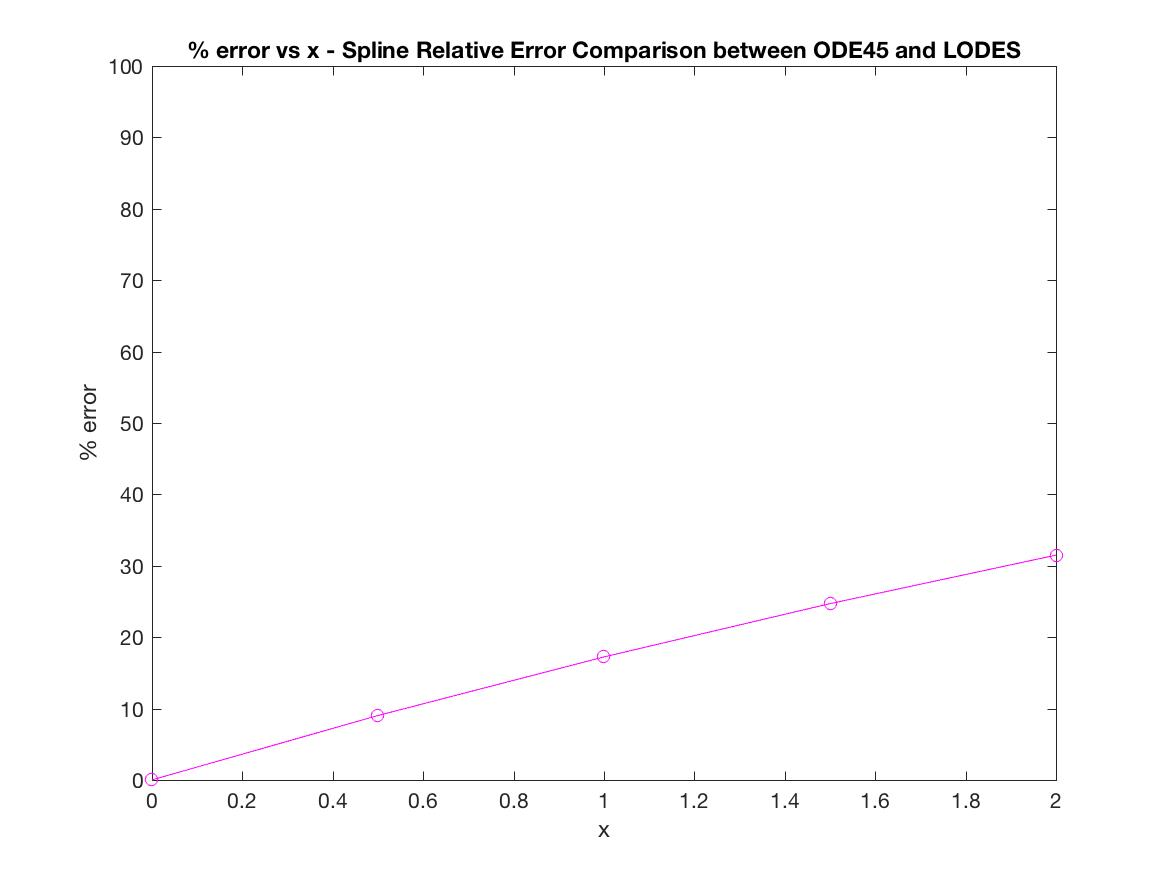
\includegraphics[width=\linewidth]{images/Test2/1RelativeErrorPlot.jpg}
  \caption{Relative Error Norm - Euler}
  \label{fig:euler2b}
\end{subfigure}
\caption{Euler's Method Analysis Graphs}
\label{fig:euler2}
\end{figure}

\begin{figure}[H]
\centering
\begin{subfigure}{.55\textwidth}
  \centering
  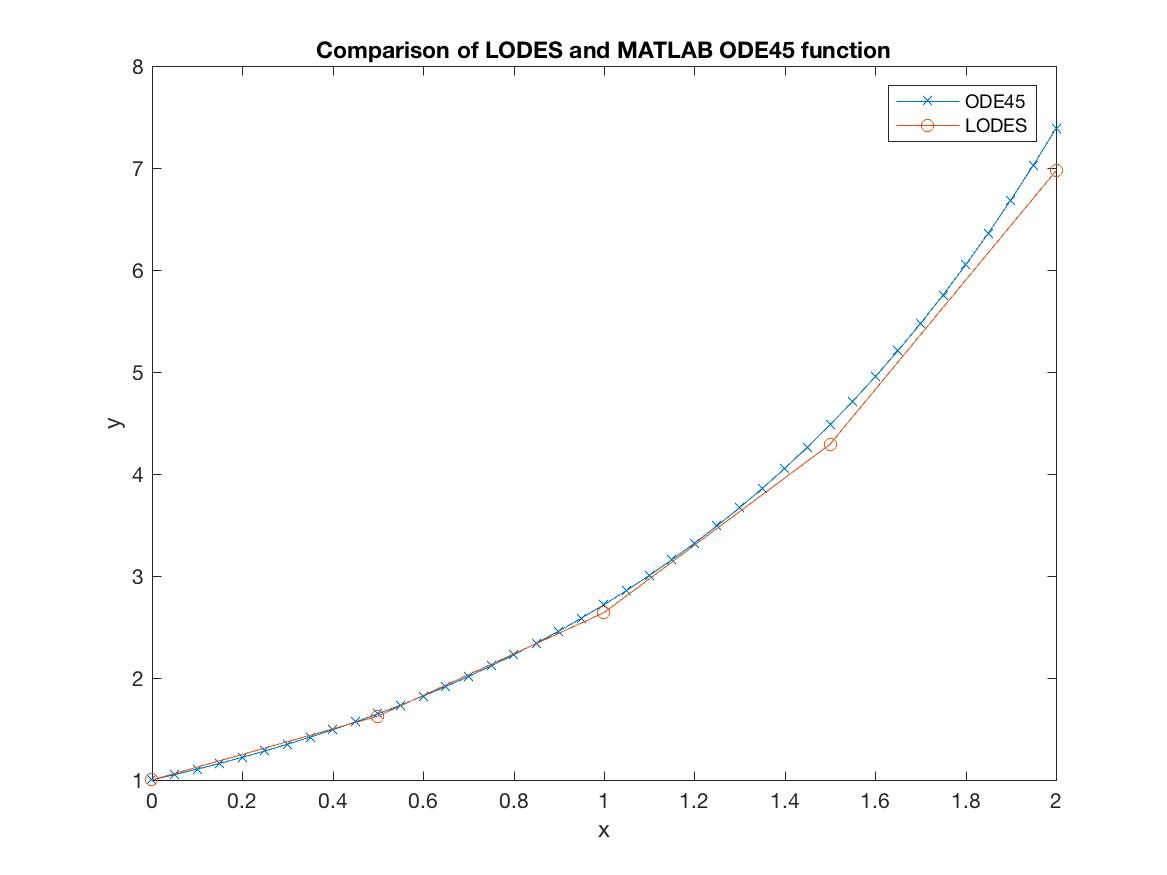
\includegraphics[width=\linewidth]{images/Test2/2LODESvsMATLABPlot.jpg}
  \caption{Trapezoid vs. ODE45}
  \label{fig:trap2a}
\end{subfigure}%
\begin{subfigure}{.55\textwidth}
  \centering
  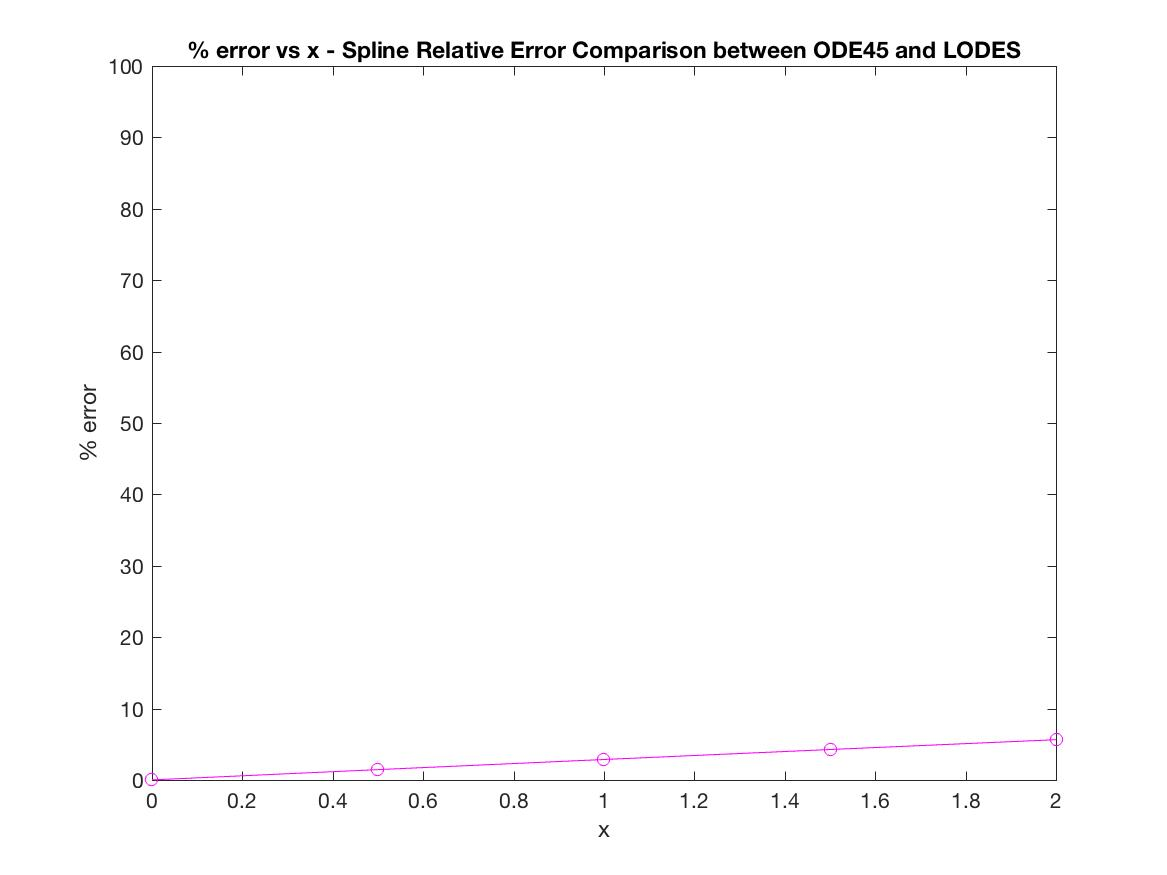
\includegraphics[width=\linewidth]{images/Test2/2RelativeErrorPlot.jpg}
  \caption{Relative Error Norm - Trapezoid}
  \label{fig:trap2b}
\end{subfigure}
\caption{Trapezoidal Method Analysis Graphs}
\label{fig:trap2}
\end{figure}

\begin{figure}[H]
\centering
\begin{subfigure}{.55\textwidth}
  \centering
  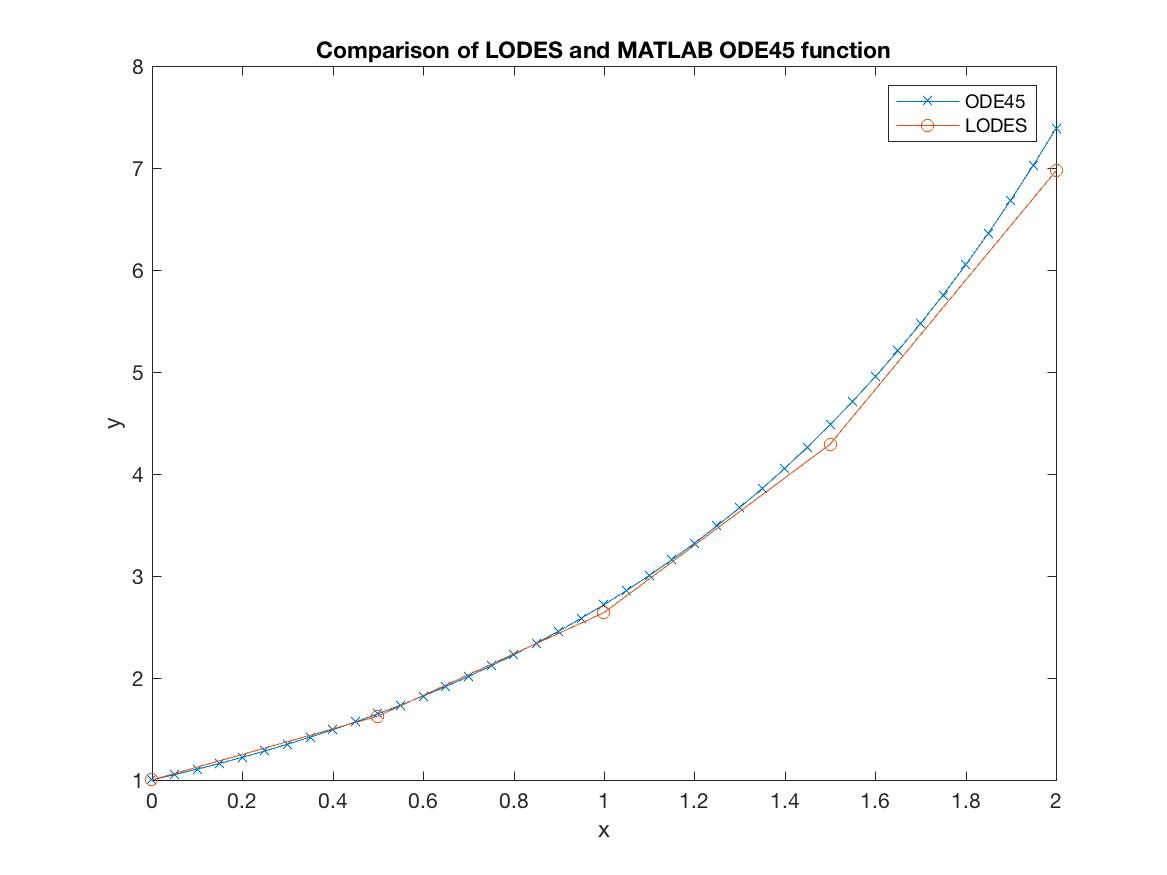
\includegraphics[width=\linewidth]{images/Test2/3LODESvsMATLABPlot.jpg}
  \caption{Heun vs. ODE45}
  \label{fig:heun2a}
\end{subfigure}%
\begin{subfigure}{.55\textwidth}
  \centering
  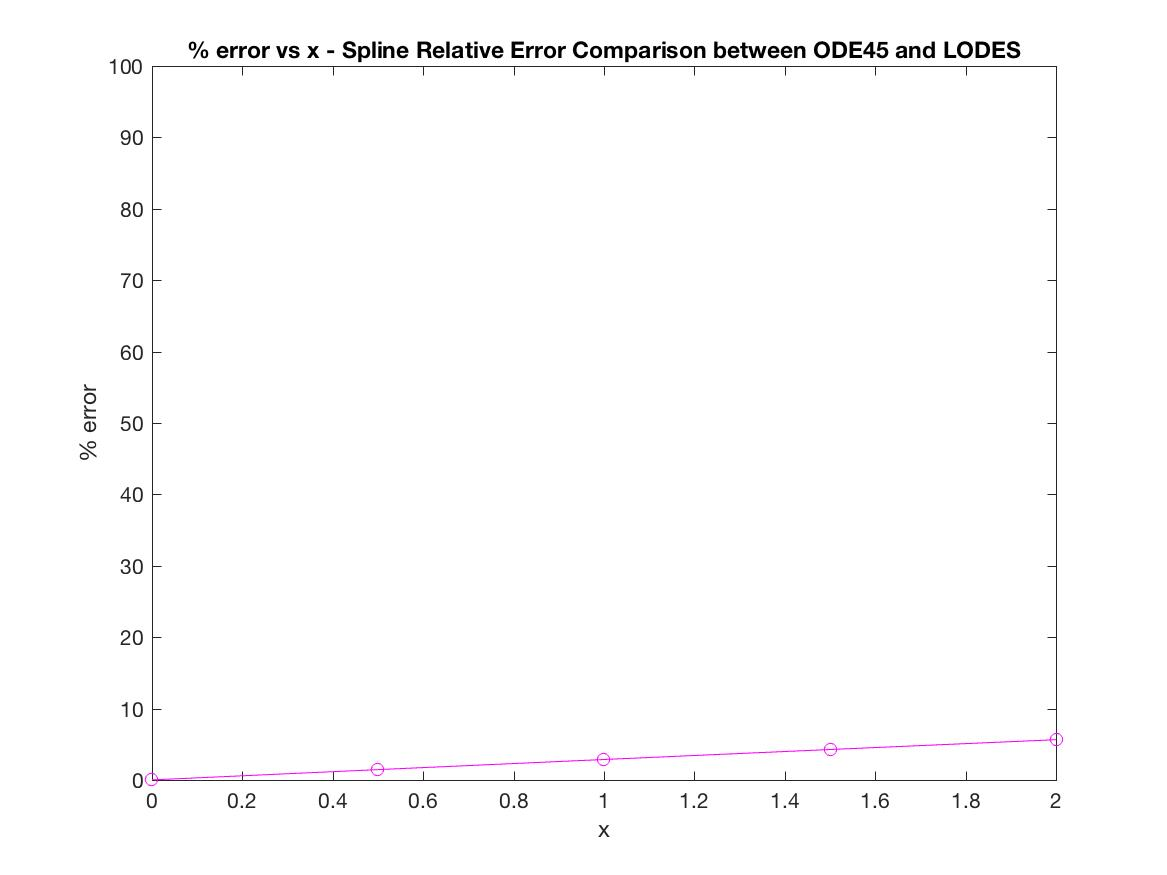
\includegraphics[width=\linewidth]{images/Test2/3RelativeErrorPlot.jpg}
  \caption{Relative Error Norm - Heun}
  \label{fig:heun2b}
\end{subfigure}
\caption{Heun's Method Analysis Graphs}
\label{fig:heun2}
\end{figure}

\begin{figure}[H]
\centering
\begin{subfigure}{.55\textwidth}
  \centering
  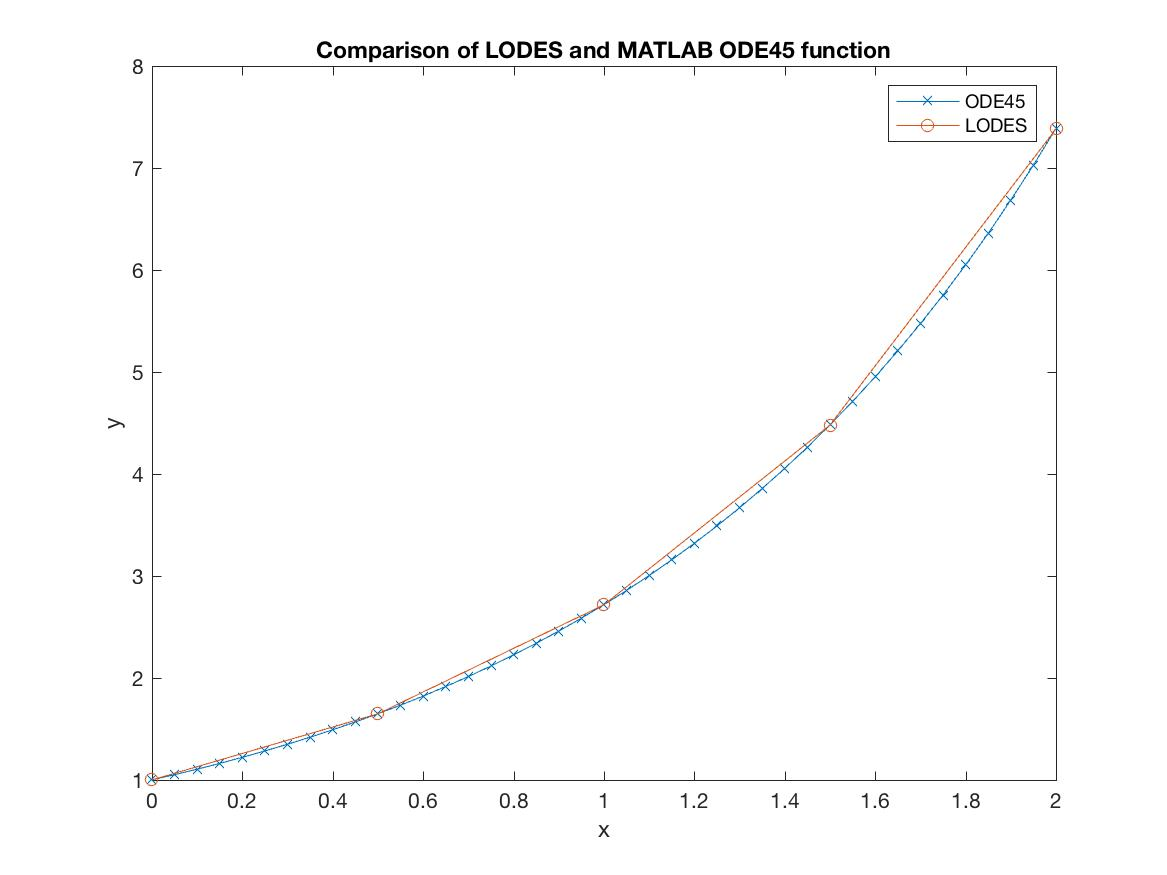
\includegraphics[width=\linewidth]{images/Test2/4LODESvsMATLABPlot.jpg}
  \caption{Runge-Kutta 4 vs. ODE45}
  \label{fig:rk2a}
\end{subfigure}%
\begin{subfigure}{.55\textwidth}
  \centering
  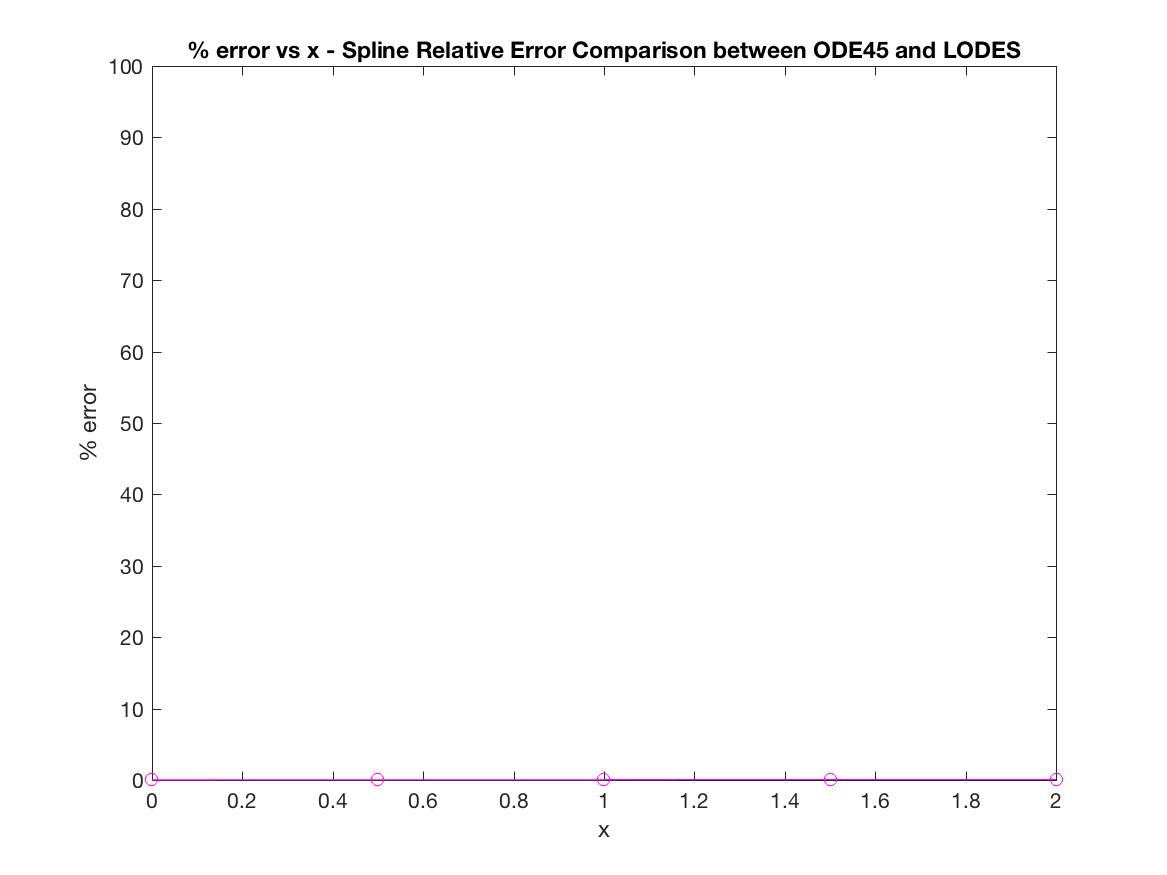
\includegraphics[width=\linewidth]{images/Test2/4RelativeErrorPlot.jpg}
  \caption{Relative Error Norm - Runge-Kutta 4}
  \label{fig:rk2b}
\end{subfigure}
\caption{Runge-Kutta 4 Method Analysis Graphs}
\label{fig:rk2}
\end{figure}







\subsection{Test 3: $f(x,y) = sin(x) - y^2, h = 5,x_0 = 0,y_0 = 1,x_k = 5$} \label{sec_t3}
\begin{figure}[H]
\centering
\begin{subfigure}{.55\textwidth}
  \centering
  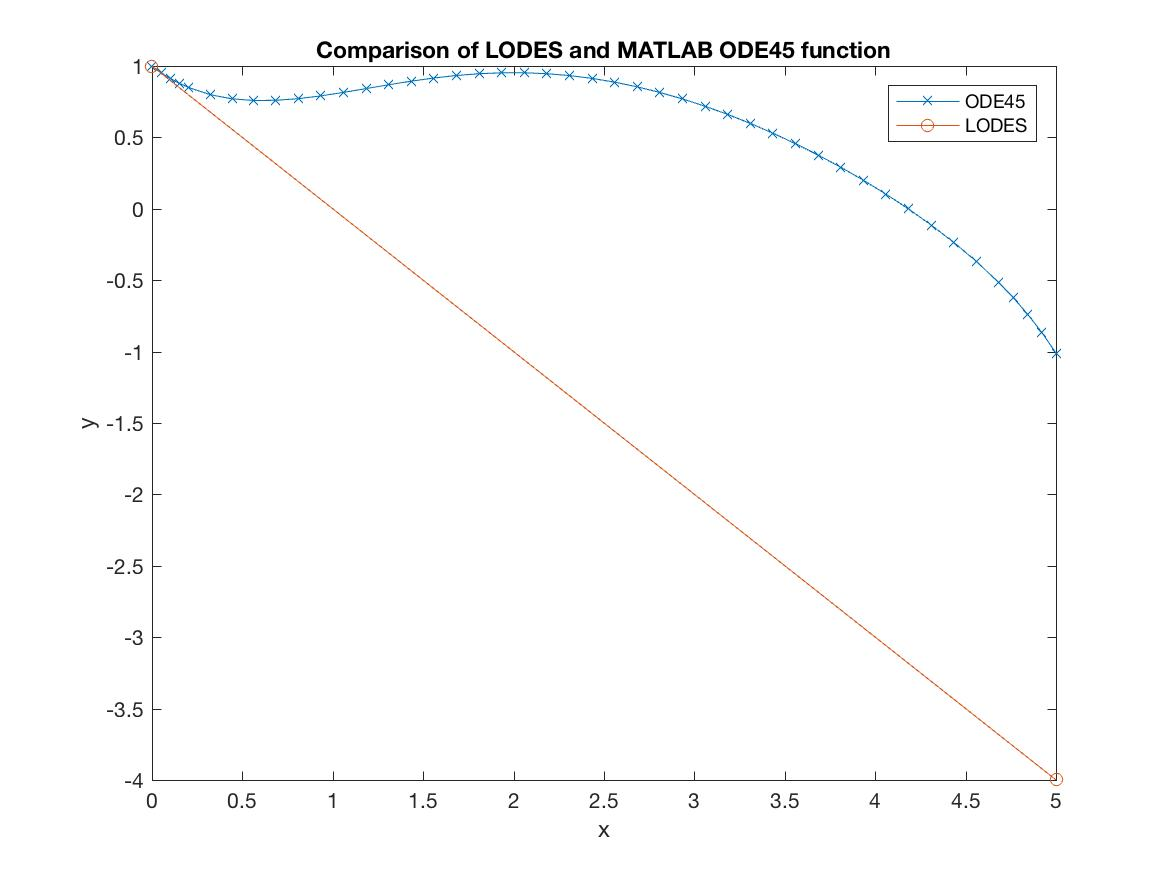
\includegraphics[width=\linewidth]{images/Test3/1LODESvsMATLABPlot.jpg}
  \caption{Euler vs. ODE45}
  \label{fig:euler3a}
\end{subfigure}%
\begin{subfigure}{.55\textwidth}
  \centering
  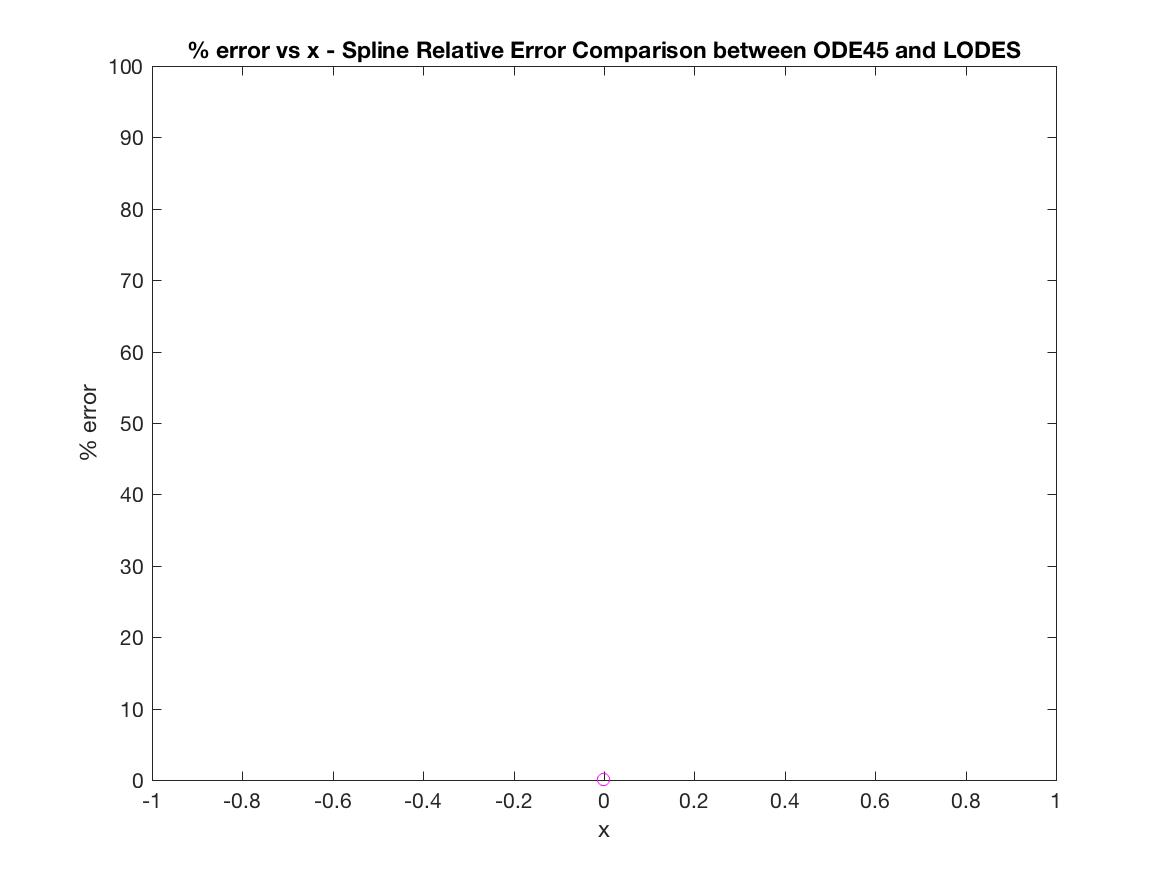
\includegraphics[width=\linewidth]{images/Test3/1RelativeErrorPlot.jpg}
  \caption{Relative Error Norm - Euler}
  \label{fig:euler3b}
\end{subfigure}
\caption{Euler's Method Analysis Graphs}
\label{fig:euler3}
\end{figure}

\begin{figure}[H]
\centering
\begin{subfigure}{.55\textwidth}
  \centering
  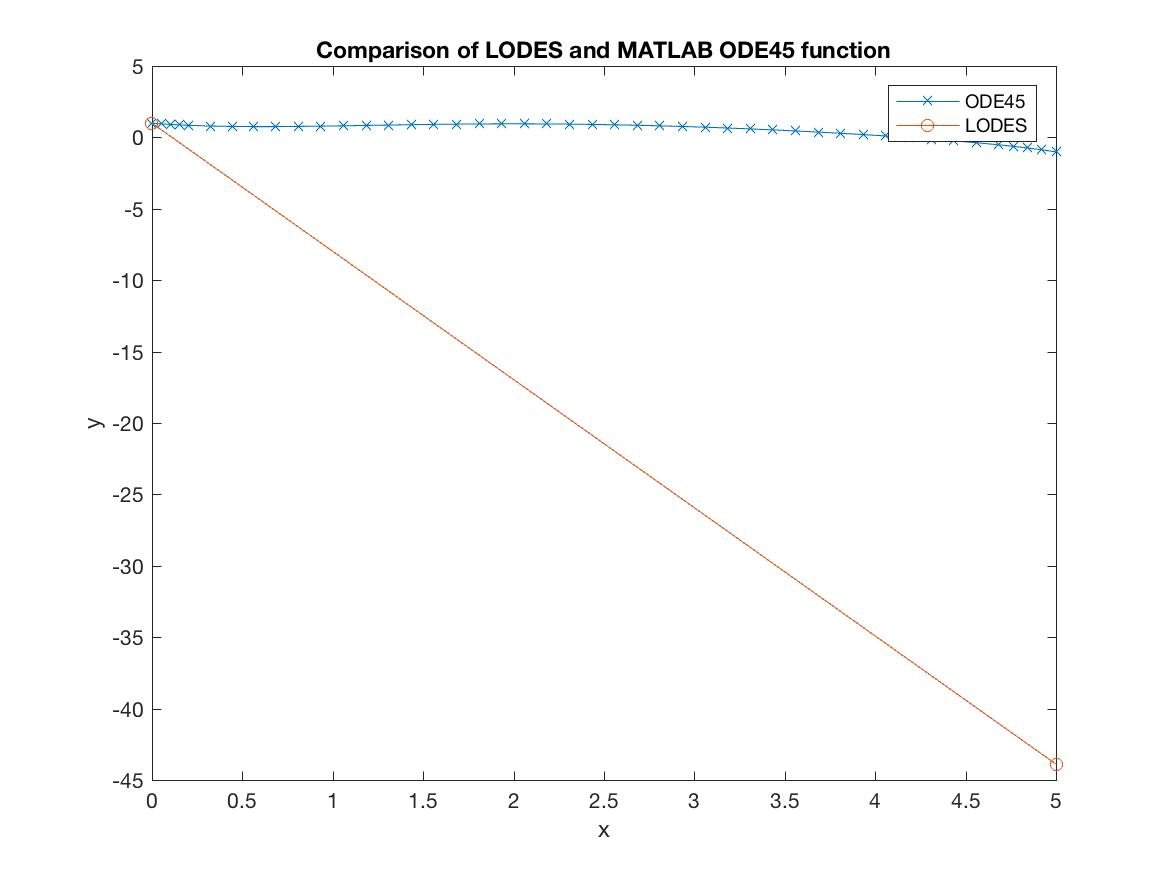
\includegraphics[width=\linewidth]{images/Test3/2LODESvsMATLABPlot.jpg}
  \caption{Trapezoid vs. ODE45}
  \label{fig:trap3a}
\end{subfigure}%
\begin{subfigure}{.55\textwidth}
  \centering
  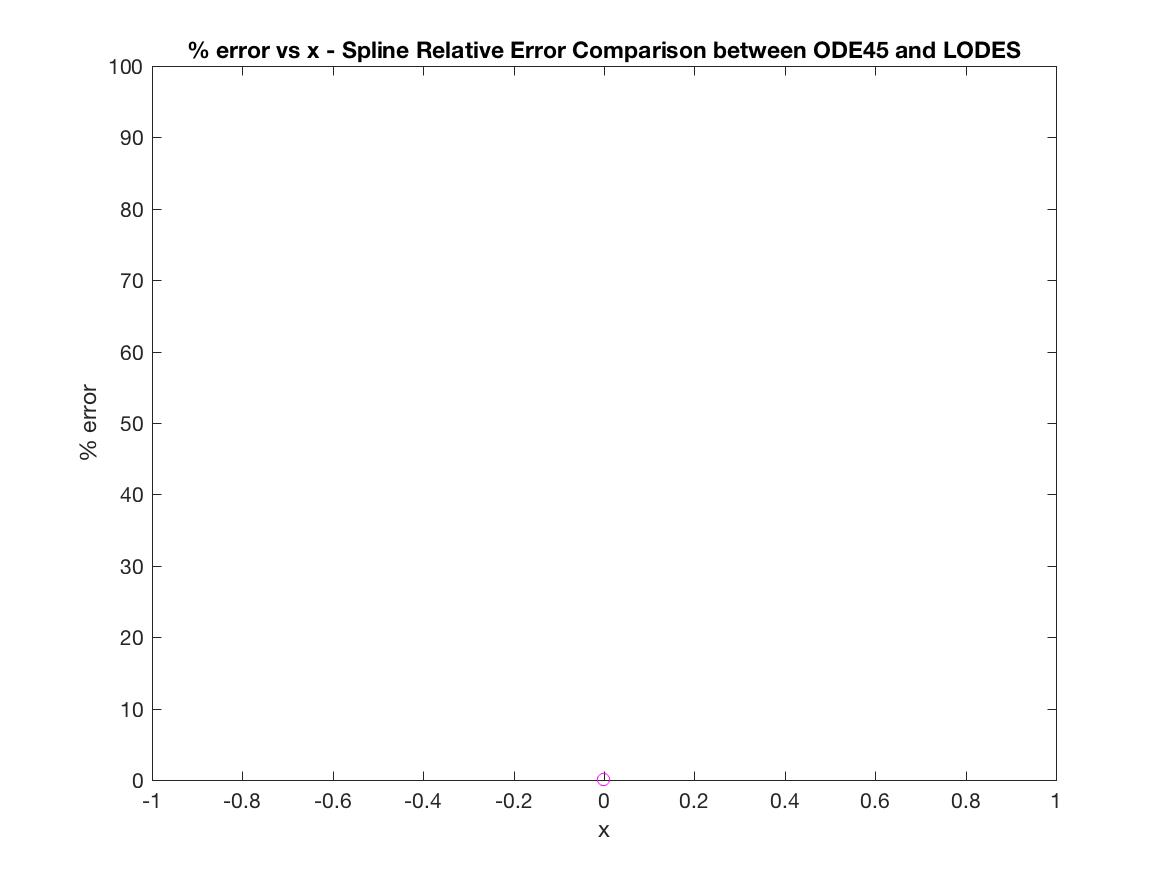
\includegraphics[width=\linewidth]{images/Test3/2RelativeErrorPlot.jpg}
  \caption{Relative Error Norm - Trapezoid}
  \label{fig:trap3b}
\end{subfigure}
\caption{Trapezoidal Method Analysis Graphs}
\label{fig:trap3}
\end{figure}

\begin{figure}[H]
\centering
\begin{subfigure}{.55\textwidth}
  \centering
  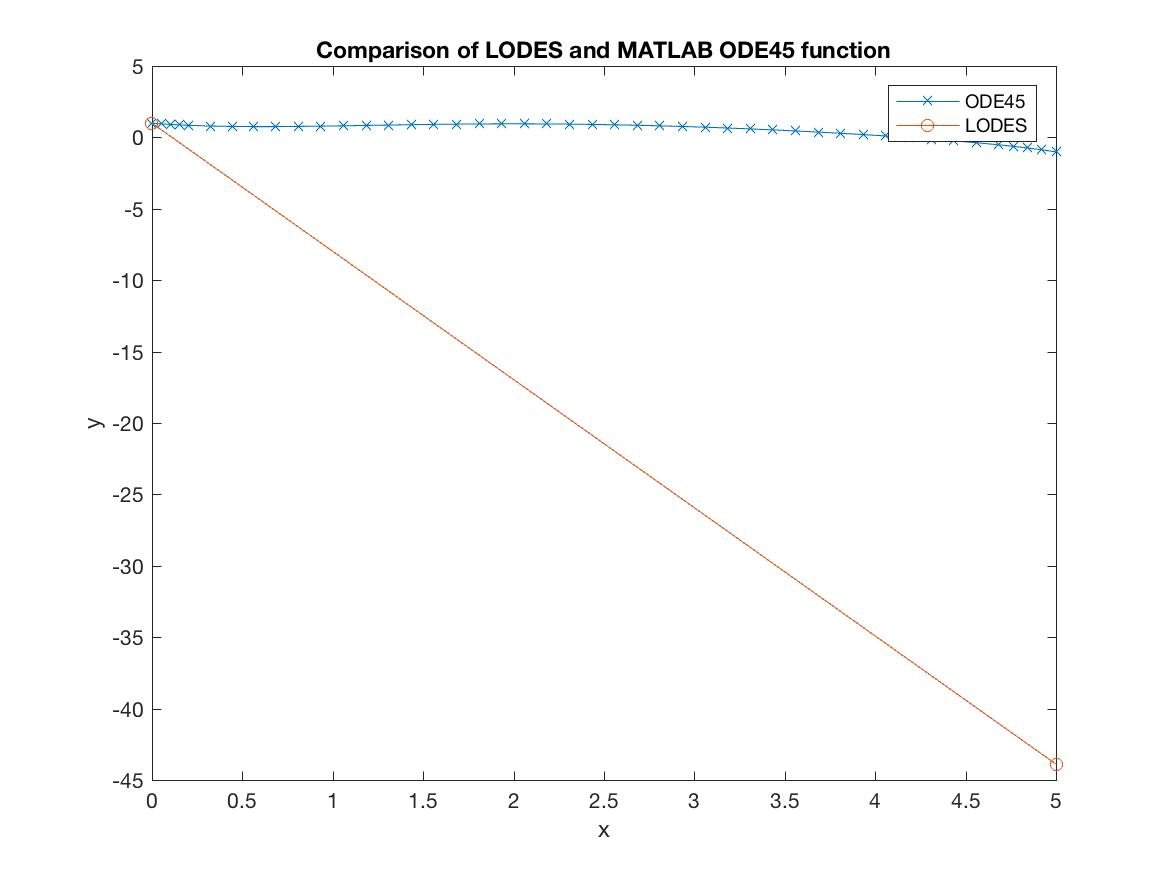
\includegraphics[width=\linewidth]{images/Test3/3LODESvsMATLABPlot.jpg}
  \caption{Heun vs. ODE45}
  \label{fig:heun3a}
\end{subfigure}%
\begin{subfigure}{.55\textwidth}
  \centering
  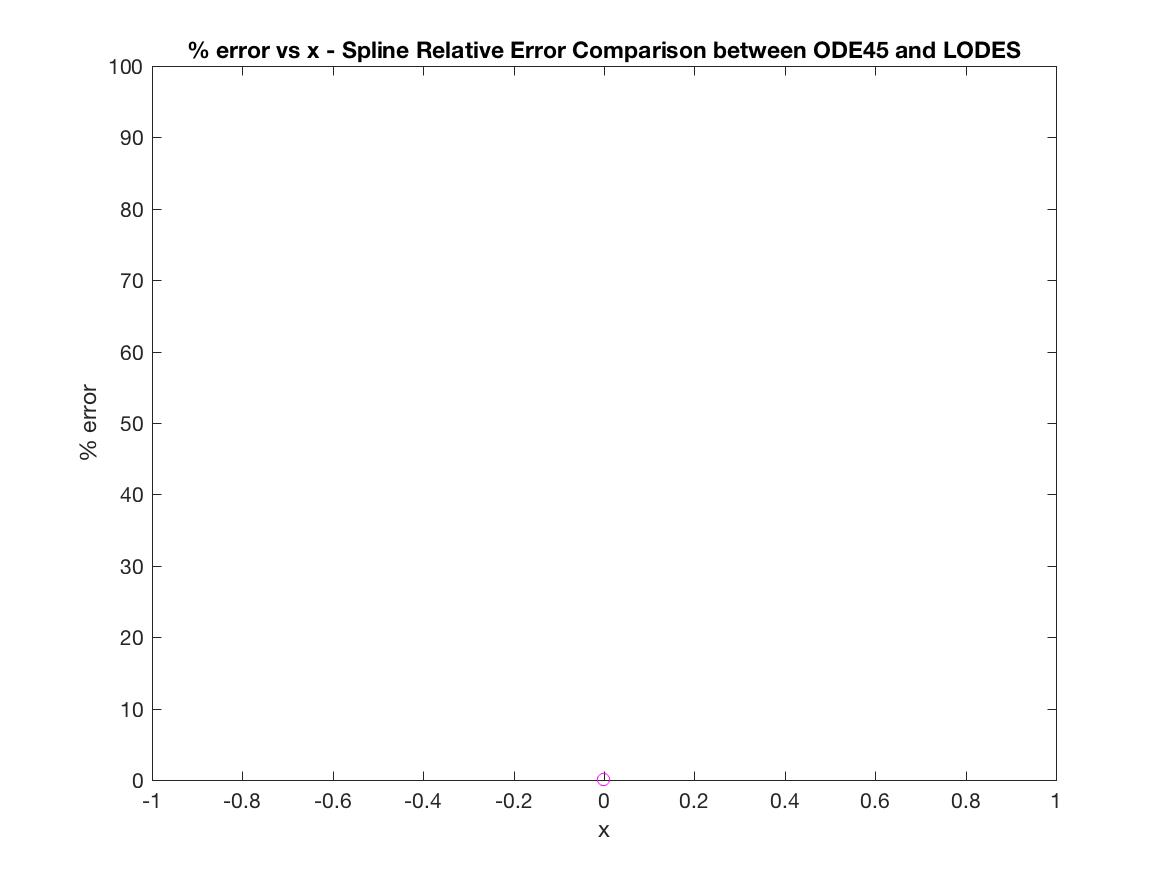
\includegraphics[width=\linewidth]{images/Test3/3RelativeErrorPlot.jpg}
  \caption{Relative Error Norm - Heun}
  \label{fig:heun3b}
\end{subfigure}
\caption{Heun's Method Analysis Graphs}
\label{fig:heun3}
\end{figure}

\begin{figure}[H]
\centering
\begin{subfigure}{.55\textwidth}
  \centering
  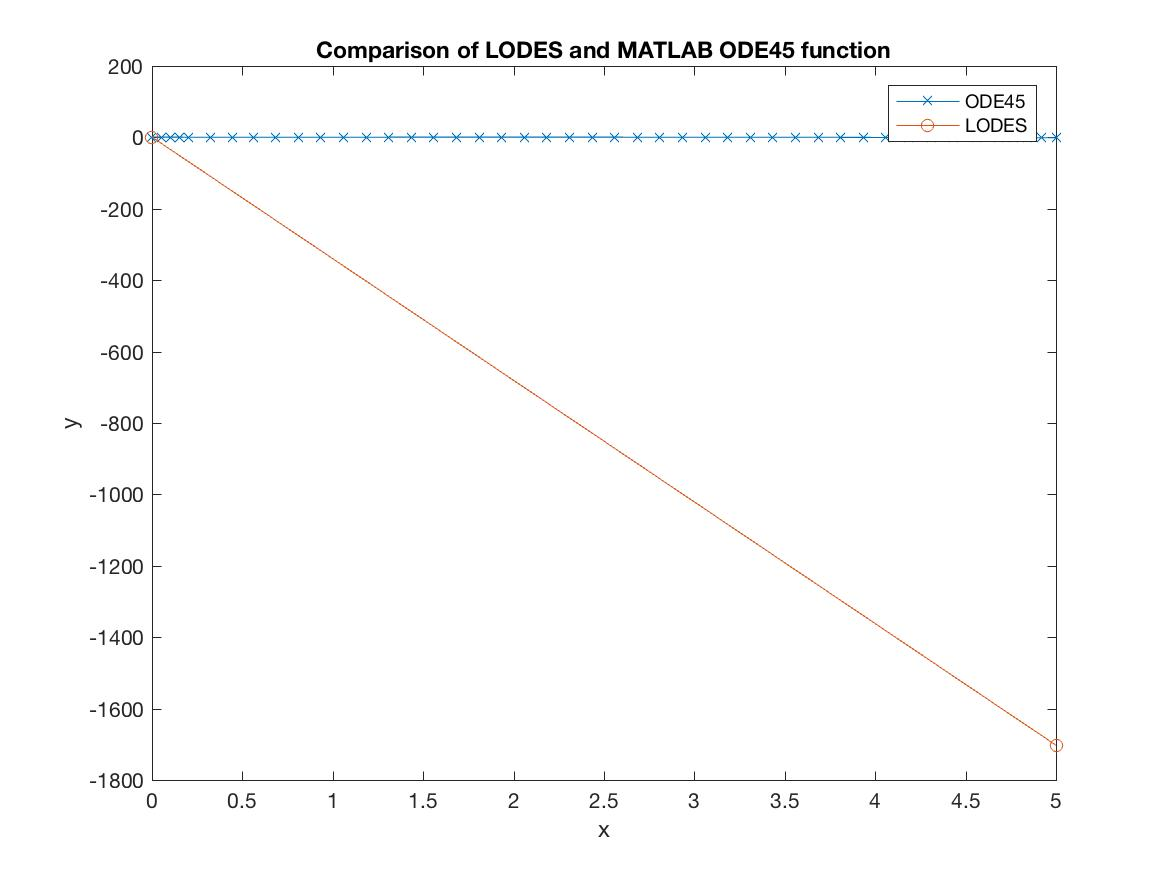
\includegraphics[width=\linewidth]{images/Test3/4LODESvsMATLABPlot.jpg}
  \caption{Runge-Kutta 4 vs. ODE45}
  \label{fig:rk3a}
\end{subfigure}%
\begin{subfigure}{.55\textwidth}
  \centering
  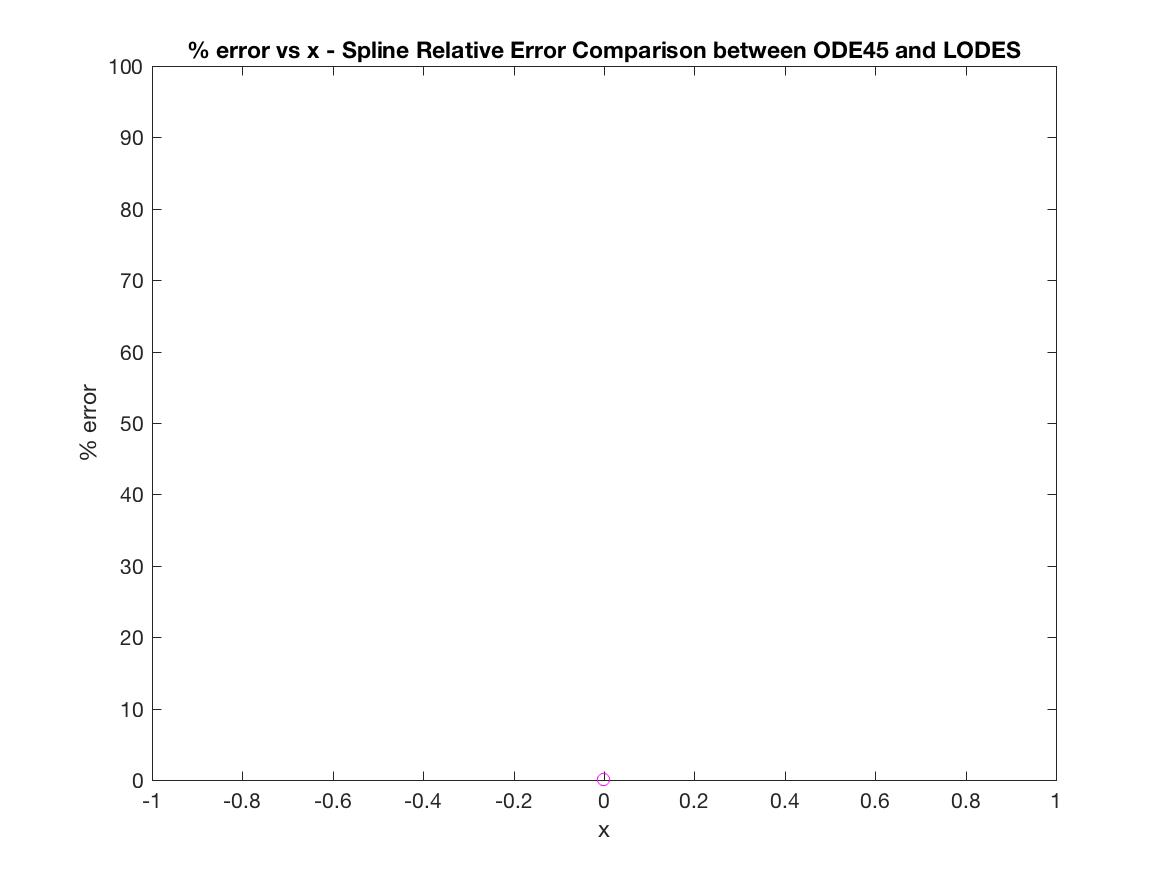
\includegraphics[width=\linewidth]{images/Test3/4RelativeErrorPlot.jpg}
  \caption{Relative Error Norm - Runge-Kutta 4}
  \label{fig:rk3b}
\end{subfigure}
\caption{Runge-Kutta 4 Method Analysis Graphs}
\label{fig:rk3}
\end{figure}





\subsection{Test 4: $f(x,y) = sin(x) - y^2, h = 1,x_0 = 0,y_0 = 1,x_k = 5$} \label{sec_t4}
\begin{figure}[H]
\centering
\begin{subfigure}{.55\textwidth}
  \centering
  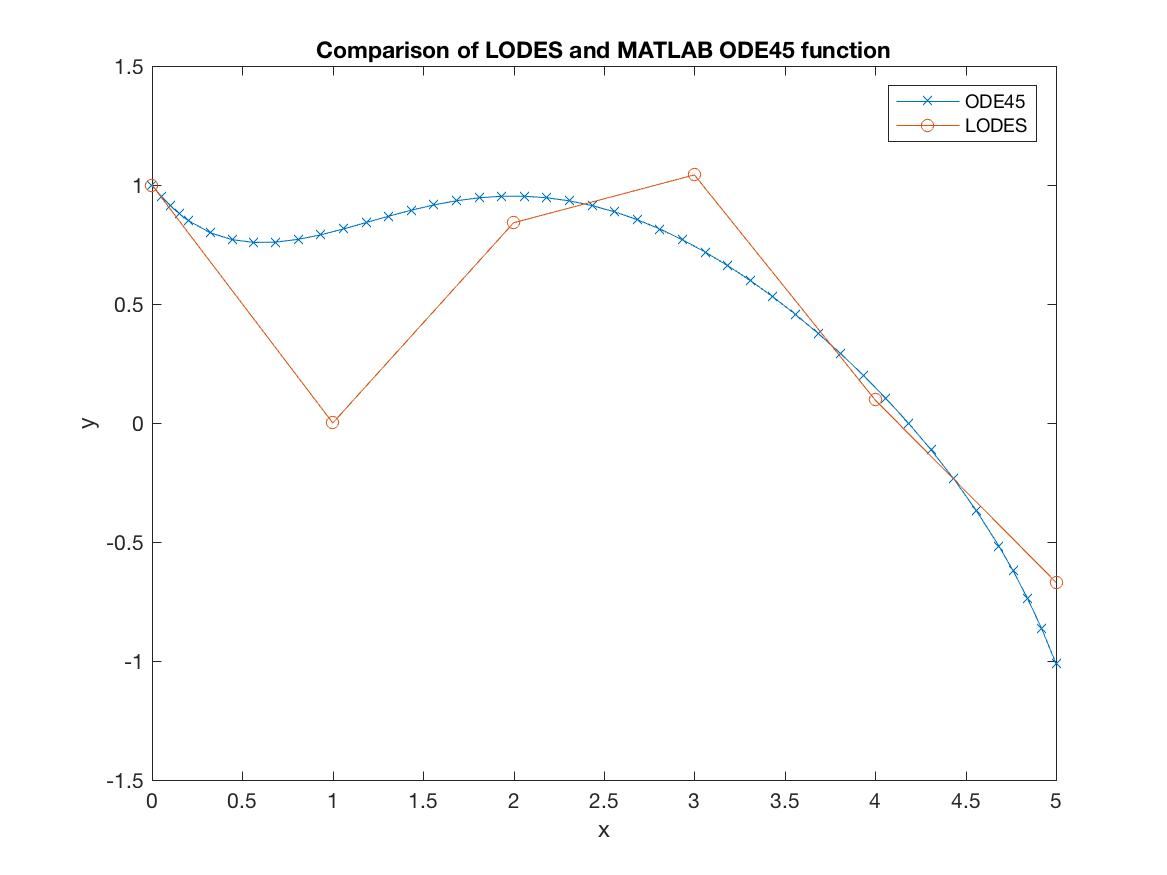
\includegraphics[width=\linewidth]{images/Test4/1LODESvsMATLABPlot.jpg}
  \caption{Euler vs. ODE45}
  \label{fig:euler4a}
\end{subfigure}%
\begin{subfigure}{.55\textwidth}
  \centering
  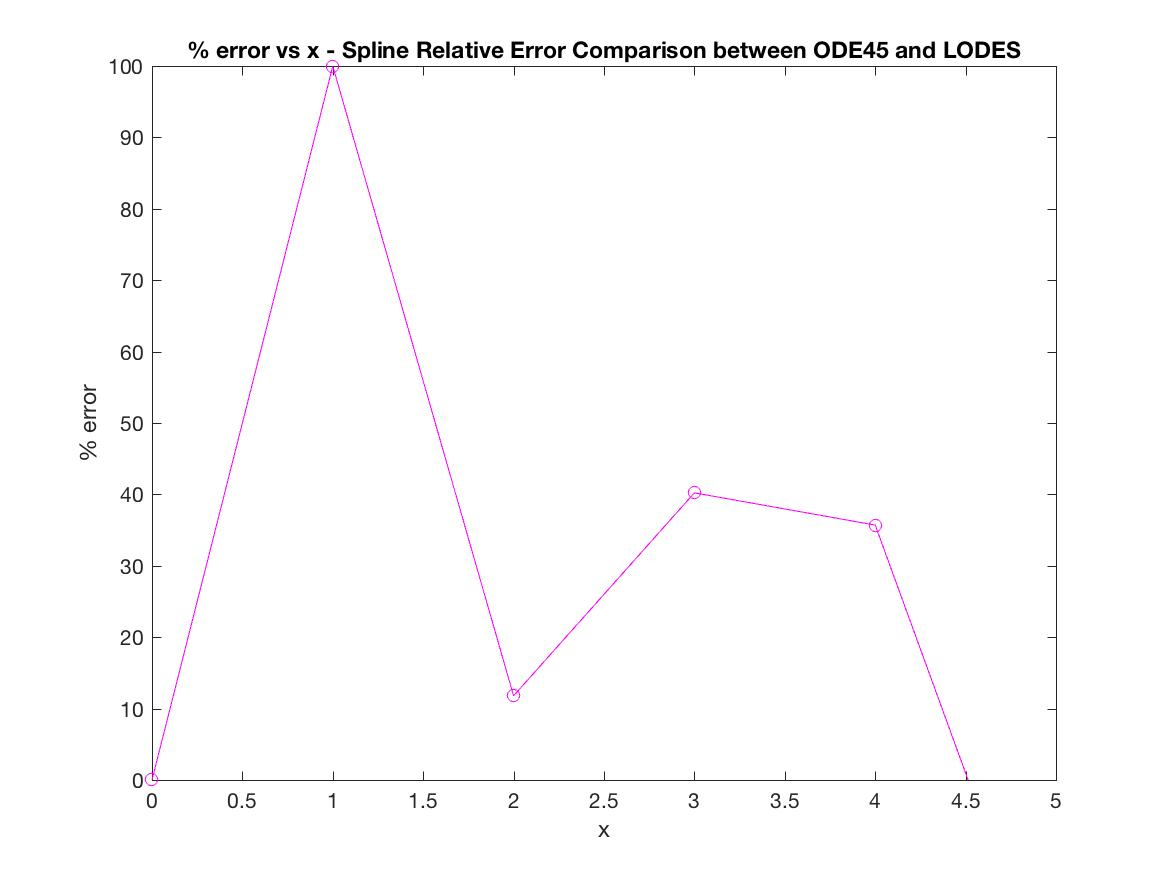
\includegraphics[width=\linewidth]{images/Test4/1RelativeErrorPlot.jpg}
  \caption{Relative Error Norm - Euler}
  \label{fig:euler4b}
\end{subfigure}
\caption{Euler's Method Analysis Graphs}
\label{fig:euler4}
\end{figure}

\begin{figure}[H]
\centering
\begin{subfigure}{.55\textwidth}
  \centering
  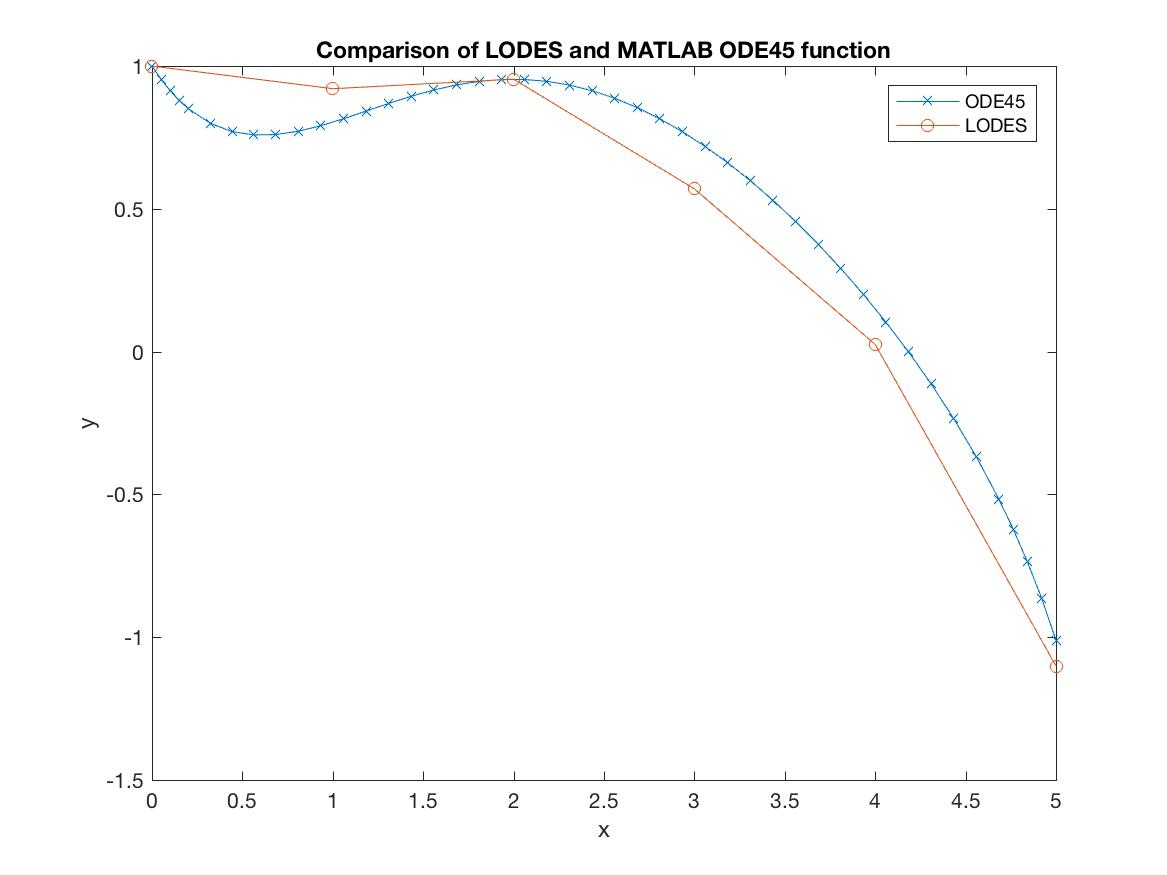
\includegraphics[width=\linewidth]{images/Test4/2LODESvsMATLABPlot.jpg}
  \caption{Trapezoid vs. ODE45}
  \label{fig:trap4a}
\end{subfigure}%
\begin{subfigure}{.55\textwidth}
  \centering
  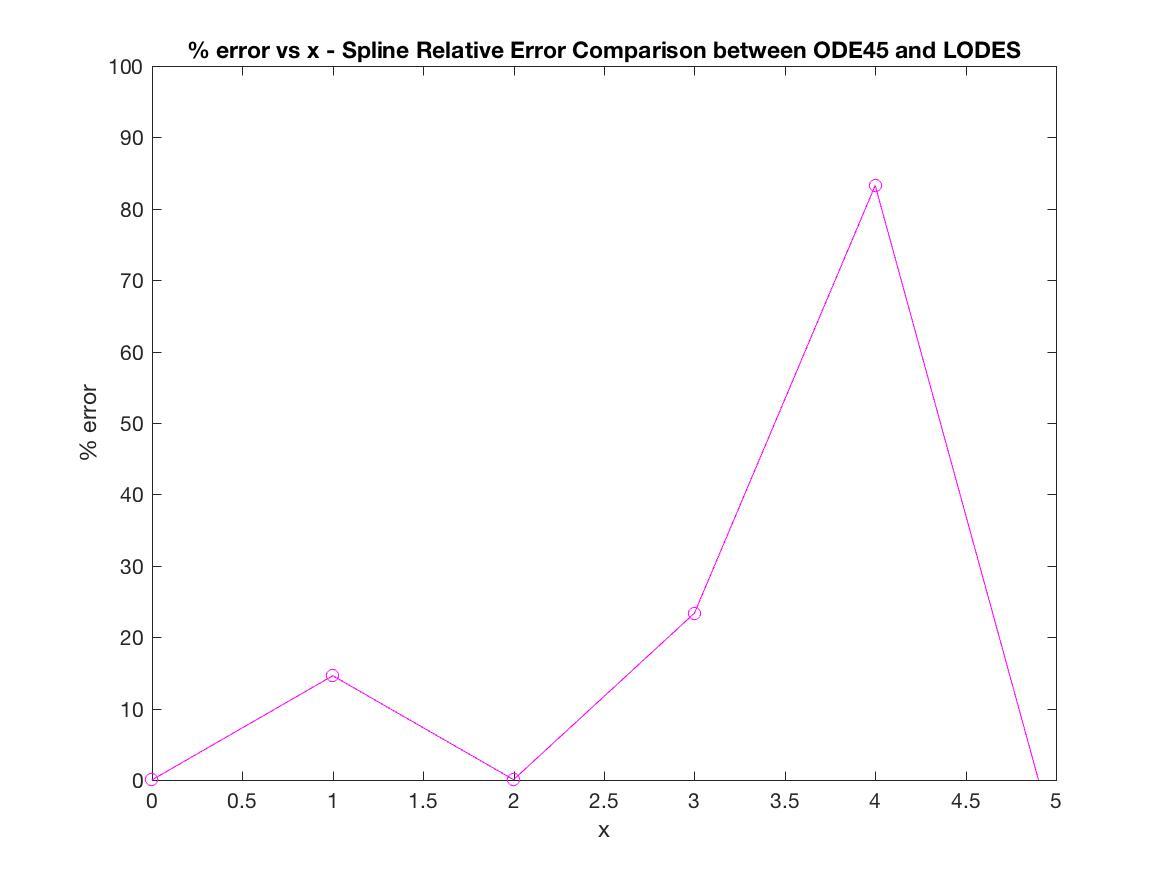
\includegraphics[width=\linewidth]{images/Test4/2RelativeErrorPlot.jpg}
  \caption{Relative Error Norm - Trapezoid}
  \label{fig:trap4b}
\end{subfigure}
\caption{Trapezoidal Method Analysis Graphs}
\label{fig:trap4}
\end{figure}

\begin{figure}[H]
\centering
\begin{subfigure}{.55\textwidth}
  \centering
  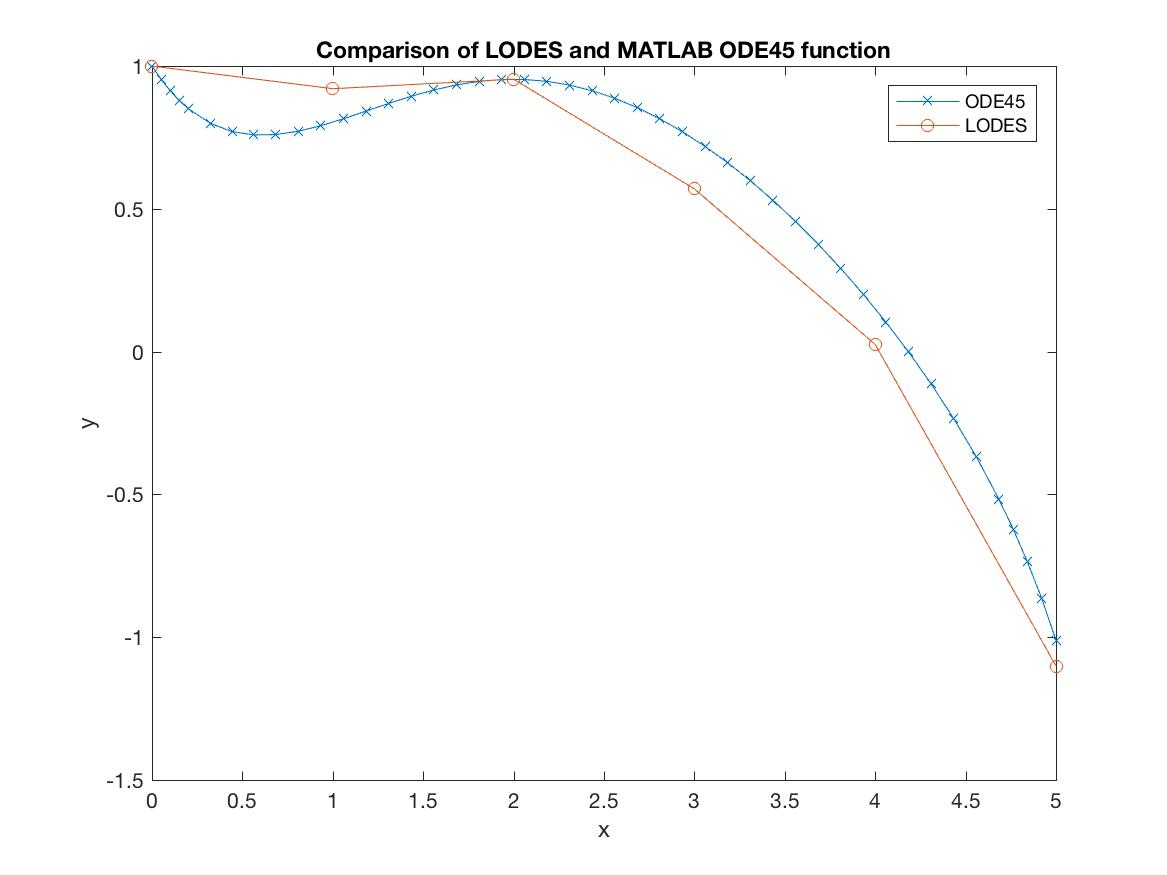
\includegraphics[width=\linewidth]{images/Test4/3LODESvsMATLABPlot.jpg}
  \caption{Heun vs. ODE45}
  \label{fig:heun4a}
\end{subfigure}%
\begin{subfigure}{.55\textwidth}
  \centering
  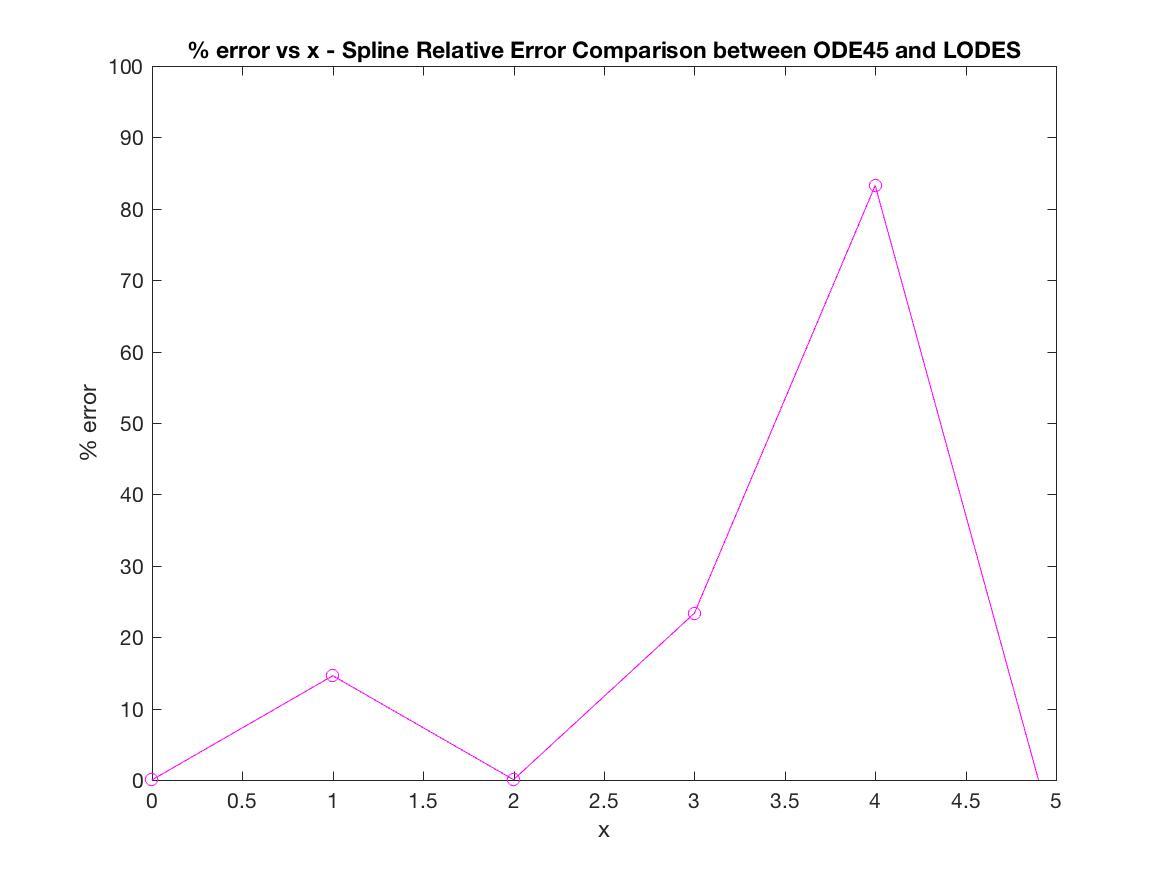
\includegraphics[width=\linewidth]{images/Test4/3RelativeErrorPlot.jpg}
  \caption{Relative Error Norm - Heun}
  \label{fig:heun4b}
\end{subfigure}
\caption{Heun's Method Analysis Graphs}
\label{fig:heun4}
\end{figure}

\begin{figure}[H]
\centering
\begin{subfigure}{.55\textwidth}
  \centering
  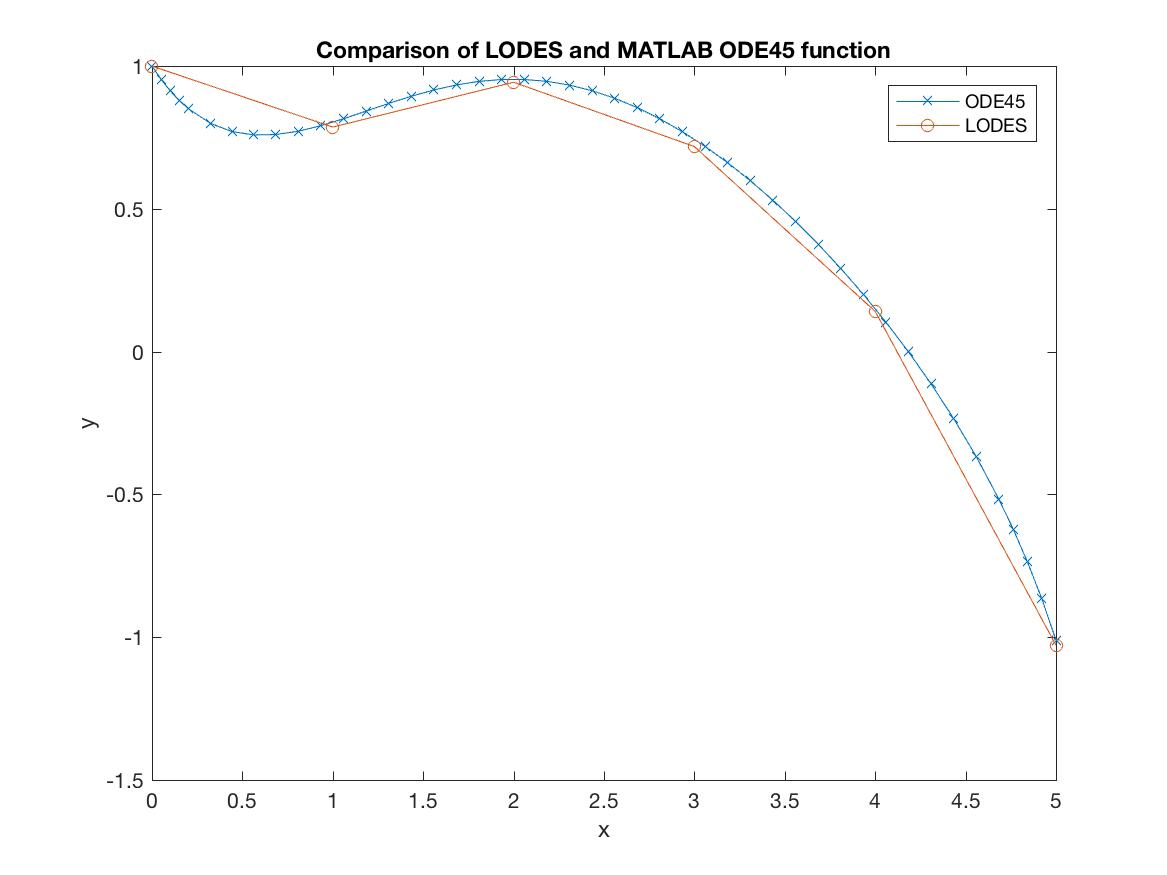
\includegraphics[width=\linewidth]{images/Test4/4LODESvsMATLABPlot.jpg}
  \caption{Runge-Kutta 4 vs. ODE45}
  \label{fig:rk4a}
\end{subfigure}%
\begin{subfigure}{.55\textwidth}
  \centering
  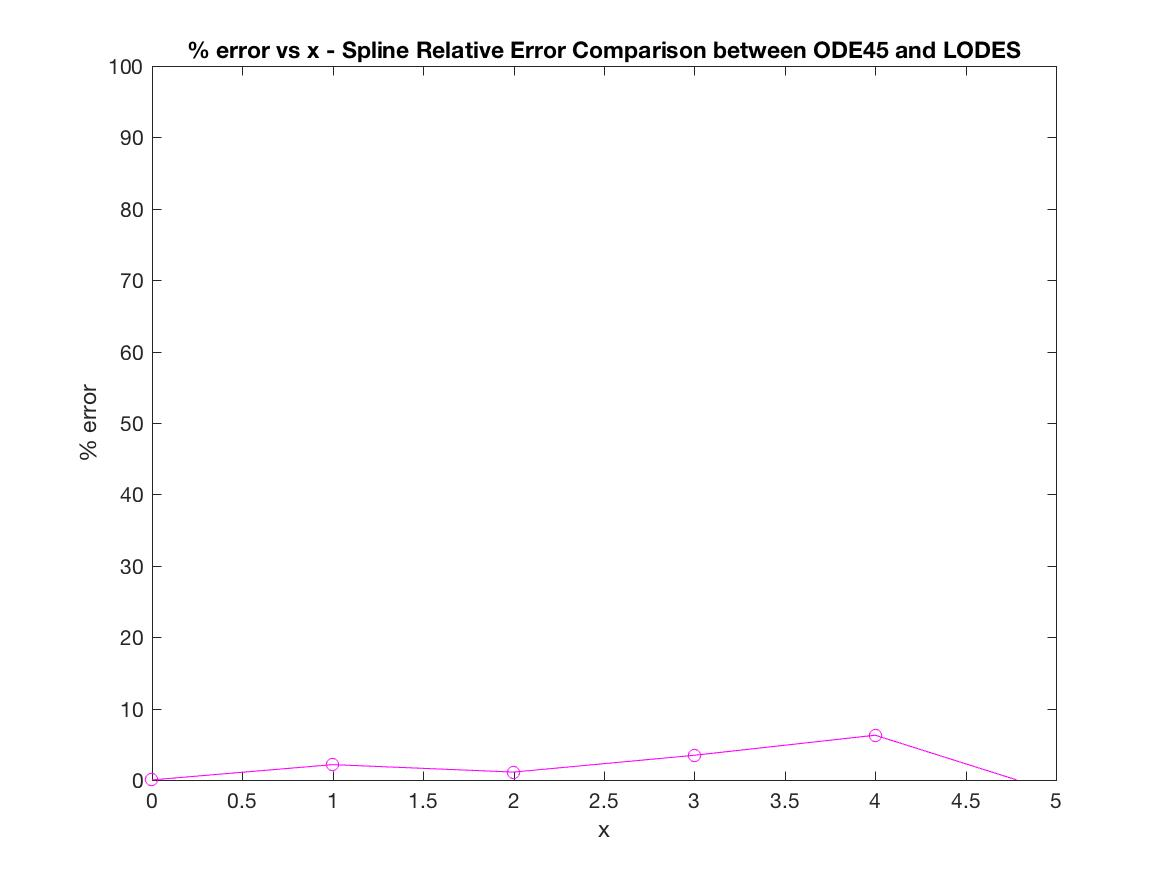
\includegraphics[width=\linewidth]{images/Test4/4RelativeErrorPlot.jpg}
  \caption{Relative Error Norm - Runge-Kutta 4}
  \label{fig:rk4b}
\end{subfigure}
\caption{Runge-Kutta 4 Method Analysis Graphs}
\label{fig:rk4}
\end{figure}

\section{Unit Testing} \label{sec_ut}
Unit testing was performed and the results and execution are the similar
on the level of Functional Requirement as described in Section \ref{sec_fr}
since the library is only of one level.\\

Further unit testing can be explored in the future.\\

Unit testing of the modules implemented by MATLAB and the Operating System (OS)
has been deemed unnecessary due to proof of use.

\section{Changes Due to Testing} \label{sec_changes}

None.

\section{Automated Testing} \label{sec_at}

Automated testing has been performed in Section \ref{sec_comp_exist_imp}.
These were implemented in MATLAB's Unit Testing Framework.
		
\section{Trace to Requirements} \label{sec_trace_req}

The following table shows the traceability mapping for the test cases laid out in this Test Report to the requirements 
described in the Commonality Analysis.

\begin{table} [H]
  \caption{Requirements Traceability Matrix}
  \label{Table:Table_Traceability_CA}  
\begin{tabular}{|c|p{8cm}|}
  \hline	
  \textbf{Test Number} & \textbf{CA Requirements}\\
  \hline 
   T1& IM1, O1, O2, O3, O4, O5\\ \hline
   T2& IM1, O1, O2, O3, O4, O5\\ \hline
   T3& IM1, O1, O2, O3, O4, O5\\ \hline
   T4& IM1, O1, O2, O3, O4, O5\\ \hline
   T5& IM2, O1, O2, O3, O4, O5\\ \hline
   T6& IM2, O1, O2, O3, O4, O5\\ \hline
   T7& IM2, O1, O2, O3, O4, O5\\ \hline
   T8& IM2, O1, O2, O3, O4, O5\\ \hline
   T9& IM3, O1, O2, O3, O4, O5\\ \hline
   T10& IM3, O1, O2, O3, O4, O5\\ \hline
   T11& IM3, O1, O2, O3, O4, O5\\ \hline
   T12& IM3, O1, O2, O3, O4, O5\\ \hline
   T13& IM4, O1, O2, O3, O4, O5\\ \hline
   T14& IM4, O1, O2, O3, O4, O5\\ \hline
   T15& IM4, O1, O2, O3, O4, O5\\ \hline
   T16& IM4, O1, O2, O3, O4, O5\\ \hline
   T17& NFR1\\ \hline
   T18& NFR2\\ \hline

\end{tabular}\\
\end{table}
		
\section{Trace to Modules}	 \label{sec_trace_modules}
The following table shows the traceability mapping for the test cases laid out in this Test Report to the
modules in the Module Guide (MG).

\begin{table} [H]
  \caption{Design Traceability Matrix}
  \label{Table:Table_Traceability_MG}  
\begin{tabular}{|c|p{8cm}|}
  \hline	
  \textbf{Test Number} & \textbf{MG Modules}\\
  \hline 
   T1& M1, M2, M3, M4, M5\\ \hline
   T2& M1, M2, M3, M4, M5\\ \hline
   T3& M1, M2, M3, M4, M5\\ \hline
   T4& M1, M2, M3, M4, M5\\ \hline
   T5& M1, M2, M3, M4, M6\\ \hline
   T6& M1, M2, M3, M4, M6\\ \hline
   T7& M1, M2, M3, M4, M6\\ \hline
   T8& M1, M2, M3, M4, M6\\ \hline
   T9& M1, M2, M3, M4, M7\\ \hline
   T10& M1, M2, M3, M4, M7\\ \hline
   T11& M1, M2, M3, M4, M7\\ \hline
   T12& M1, M2, M3, M4, M7\\ \hline
   T13& M1, M2, M3, M4, M8\\ \hline
   T14& M1, M2, M3, M4, M8\\ \hline
   T15& M1, M2, M3, M4, M8\\ \hline
   T16& M1, M2, M3, M4, M8\\ \hline
   T17& - \\ \hline
   T18& - \\ \hline

\end{tabular}\\
\end{table}

\section{Code Coverage Metrics} \label{sec_ccm}
The following Code Coverage figure was obtained from MATLAB's 
Code Coverage Report Tool. Running the test program with in-boundary
conditions (excluding extraneous scenarios), the code coverage tool
produces the following results:\\

\begin{figure}[H]
 \includegraphics[width=\linewidth]{images/CCM}
  \caption{Code Coverage Tool result.}
  \label{fig:CCM}
\end{figure}

\bibliographystyle{plainnat}

\bibliography{SRS}

\newpage
\begin{landscape}
\section{Appendix A - Test Output} \label{app_a}
\lstinputlisting[breaklines]{automatedtestoutput.txt}
\end{landscape}
\end{document}
